\documentclass[letterpaper,12pt]{article}
\usepackage{matharticle}
\usepackage{graphtheory}
\usepackage{flowchart}
\usepackage{afterpage}
\usepackage{url}
\usepackage{graphicx}
\usetikzlibrary{arrows}
\pagestyle{plain}
\newcommand{\sR}{\mathscr{R}}
\newcommand{\coloring}[1]{\(#1\)-coloring}
\newcommand{\colorable}[1]{\(#1\)-colorable}
\newcommand{\chromatic}[1]{\(#1\)-chromatic}
\newcommand{\clique}[1]{\(#1\)-clique}
\newcommand{\X}{\chi}
\renewcommand{\a}{\alpha}
\renewcommand{\d}{\delta}
\newcommand{\D}{\Delta}
\renewcommand{\l}{\lambda}
\newcommand{\w}{\omega}
\newcommand{\SG}{\mathscr{G}}
\newcommand{\BO}{\mathcal{O}}
\newtheorem{proposition}{Proposition}
\newtheorem{axiom}{Axiom}
\newcommand{\restrict}[2]{#1\raise-0.5ex\hbox{\ensuremath|}_{#2}}
\newcommand{\FR}{\text{FR}}
\newcommand{\DP}{\text{DP}}
\newcommand{\txtclr}[1]{\textcolor{#1}{#1}}
\newcommand{\mtxtclr}[1]{\text{\txtclr{#1}}}
\allowdisplaybreaks
\begin{document}

\title{Determining a Graph's Chromatic Number for Part Consolidation in Axiomatic Design}
\author{Jeffery A. Cavallaro\\
  Graduate Student\\
  Mathematics Department\\
  San Jose State University\\
  \url{jeffery.cavallaro@sjsu.edu}}

\maketitle

\section{Axiomatic Design}

The axiomatic design framework was developed in the late \(20^{th}\) century by Professor Nam P. Suh while at MIT
and the NSF \cite{suh}.  This was in response to concern in the engineering community that \emph{design} was being
practiced almost exclusively as an ad-hoc creative endeavor with very little in the way of scientific discipline.
In the words of Professor Suh:
\begin{quote}
  It [design] might have preceding the development of natural sciences by scores of centuries.  Yet, to this day,
  design is being done intuitively as an art.  It is one of the few technical areas where experience is more
  important than formal education.
\end{quote}
It is important to note that Professor Suh was not making these claims in an educational vacuum, but in the shadow
of several recent major design failures such as the Union Carbide plant disaster in India, nuclear power plant
accidents at Three Mile Island and Chenobyl, and the Challenger space shuttle O-ring failure.  Furthermore,
Professor Suh asserts that design-related issues resulting in production problems and operating failures were
increasingly happening in everything from consumer products to big-ticket items.

The following sections provide an overview of axiomatic design as specified in detail by Professor Suh in \cite{suh},
and summarized in \cite{cavallaro,jahanbekam,suh2}.  Following is a description of how the proposed algorithm can be
a helpful tool to a designer using the axiomatic design framework.

\subsection{Design}

\emph{Design} is defined as the process by which it is determined \emph{what} needs to be achieved and then
\emph{how} to achieve it.  Thus, the decisions on what do to are just as important as how to do it.  Creativity is
the process by which experience and intuition are used to generate solutions to perceived needs.  This includes
pattern matching to and adapting existing solutions and synthesizing new solutions.  Thus, creativity plays a vital
role in design.  Since different designers may approach the same problem differently, their level of creativity may
lead to very different, yet plausible, solutions.  Thus, there needs to be a design-agnostic method for comparing
different designs with the goal of selecting the best one.

This discussion will sound very familiar to mathematicians, since creativity is very important for solving math
problems, and in particular, for writing proofs.  Starting with the work of Peano in the \(19^{th}\) century, the
field of mathematics has established various tests on what constitutes a good proof.  For example:
\begin{itemize}
\item Does every conclusion result by proper implication from existing definitions, axioms, and previously-proved
  conclusions?
\item Is direct proof, contrapositive proof, proof by contradiction, or proof by induction the best approach for a
  particular problem?
\item Do proofs by induction contain clear basic, assumptive, and inductive steps?
\item Are all subset and equality relationships properly proved via membership implication?
\item Are all necessary cases included and stated in a mutually exclusive manner?
\item Are all equivalences proved in a proper circular fashion?
\item Are key and reused conclusions highlighted in lemmas?
\end{itemize}
In short, Professor Suh was looking for a similar framework for the more general concept of design.

\subsection{The Framework}

In a desire to not hinder the creative element needed for design, yet provide some methodology to distinguish bad
designs from good designs from better designs, the diagram in Figure \ref{fig:design} establishes the overall
framework for axiomatic design.

\begin{figure}[h]
  \label{fig:design}
  \begin{center}
    \scalebox{0.75}{
      \begin{tikzpicture}[>=latex',every text node part/.style={align=center}]
        \node (cn) [draw,terminal] at (0,0) {customer \\ needs};
        \node (pd) [draw,process,right=of cn] {problem \\ definition};
        \node (cp) [draw,process,right=2cm of pd] {creative \\ process};
        \node (ap) [draw,process,right=2cm of cp] {analytical \\ process};
        \node (uc) [draw,process,right=of ap] {ultimate \\ check};
        \node (fd) [draw,terminal,right=of uc] {final \\ design};
        \draw [->] (cn) -- (pd);
        \draw [->] (pd) -- node [auto] {FRs} (cp);
        \draw [->] (cp) -- node [auto] {candidate \\ design} (ap);
        \draw [->] (ap) -- (uc);
        \draw [->] (uc) -- (fd);
        \draw [->] (ap) -- ($(ap) + (0,-1.5cm)$) -| (cp);
      \end{tikzpicture}
    }
  \end{center}
  \caption{Axiomatic Design Framework}
\end{figure}

Design starts with the desire to fulfill a clear set of \emph{customer needs}.  The term \emph{customer} refers to
any entity that expresses needs, and can be as varied as individuals, organizations, or society.  The designer, in
the \emph{problem definition} phase, determines how these customer needs will be meet by generating a list of
\emph{functional requirements} (FRs).  It is this list of FRs that determines exactly \emph{what} is to be
accomplished.

Once the set of FRs has been determined, the designer begins the \emph{creative process} by mapping the FRs into
solutions that are embodied in so-called \emph{design parameters} (DPs).  The design parameters contain all of the
information on \emph{how} the various FRs are fulfilled: parts lists, drawings, specifications, etc.  This process
is represented by Figure \ref{fig:mapping}.

\begin{figure}[h]
  \label{fig:mapping}
  \begin{center}
    \begin{tikzpicture}[>=latex',every text node part/.style={align=center}]
      \node (fs) [draw,cloud] at (0,0) {FR1 \\ FR2 \\ FR3 \\ \vdots};
      \node [below=1ex of fs] {functional \\ space};
      \node (ps) [draw,cloud,right=1.5in of fs] {DP1 \\ DP2 \\ DP3 \\ \vdots};
      \node [below=1ex of ps] {physical \\ space};
      \draw [->] (fs) to [bend left=45] (ps);
      \draw [->] (fs) to [bend left=30] (ps);
      \draw [->] (fs) to [bend right=30] (ps);
      \draw [->] (fs) to [bend right=45] (ps);
      \draw [->] (fs) -- node [auto] {mapping} (ps);
    \end{tikzpicture}
  \end{center}
  \caption{Mapping FRs to DPs}
\end{figure}

The FRs exist in a design-agnostic \emph{functional space} and the DPs exist in a solution-specific
\emph{physical space}.  It is the designer's job to provide the most efficient mapping between the two spaces.

The FR/DP mapping is described by the \emph{design equation}, which is shown in Equation \ref{equ:design}.
\begin{equation}
  \label{equ:design}
  [\text{FR}]=[\text{A}][\text{DP}]
\end{equation}
The design equation is a matrix equation that maps a vector of \(m\) FRs to a vector of \(n\) DPs via an \(m\times
n\) design matrix A.  As will be shown, good designs require \(m=n\), and thus the design matrix is a square
\(n\times n\) matrix.  A full discussion of the design matrix element values is beyond the scope of this research.
Instead, we will use the following two values:
\[A_{ij}=\begin{cases}
X, & \text{FR}_i\ \text{depends on DP}_j \\
0, & \text{FR}_i\ \text{does not depend on DP}_j
\end{cases}\]

Since the FR/DP mapping is non-unique, there needs to be a method to compare different plausible designs so that
the best design can be selected as the final design.  Thus, the framework in Figure \ref{fig:design} includes an
\emph{analytical process} where designs are judged by a set of axioms, corollaries, and theorems that specify the
properties common to all good designs.  Once the best design, according to this analysis, is selected, it undergoes
an \emph{ultimate check} to make sure that it sufficiently meets all of the customer's needs.  If so, then that
design is selected as the final design.

\subsection{The Axioms}

The independence axiom imposes a restriction on the FR/DP mapping:

\begin{axiom}[Independence]
  \label{axm:independ}
  An optimal design always maintains the independence of the FRs.  This means that the FRs and DPs are related in
  such a way that a specific DP can be adjusted to satisfy its corresponding FR without affecting other FRs.
\end{axiom}

\begin{figure}[h]
  \label{fig:coupling}
  \scalebox{0.75}{
    \begin{minipage}{3in}
      \begin{center}
        \[\begin{bmatrix}
        FR1 \\ FR2 \\ FR3
        \end{bmatrix}=\begin{bmatrix}
        X & 0 & 0 \\
        0 & X & 0 \\
        0 & 0 & X \\
        \end{bmatrix}\begin{bmatrix}
          DP1 \\ DP2 \\ DP3
        \end{bmatrix}\]
        Uncoupled
      \end{center}
    \end{minipage}
    \begin{minipage}{3in}
      \begin{center}
        \[\begin{bmatrix}
        FR1 \\ FR2 \\ FR3
        \end{bmatrix}=\begin{bmatrix}
        X & 0 & 0 \\
        X & X & 0 \\
        X & X & X \\
        \end{bmatrix}\begin{bmatrix}
          DP1 \\ DP2 \\ DP3
        \end{bmatrix}\]
        Decoupled
      \end{center}
    \end{minipage}
    \begin{minipage}{3in}
      \begin{center}
        \[\begin{bmatrix}
        FR1 \\ FR2 \\ FR3
        \end{bmatrix}=\begin{bmatrix}
        X & X & X \\
        X & X & X \\
        X & X & X \\
        \end{bmatrix}\begin{bmatrix}
          DP1 \\ DP2 \\ DP3
        \end{bmatrix}\]
        Coupled
      \end{center}
    \end{minipage}
  }
  \caption{Coupling Examples}
\end{figure}

\subsection{Part Consolidation}

One particular area of design focus is the number of parts in a product design:
\begin{quote}
  Poorly designed products often cost more because they use more materials or parts than do well-designed products.
  They are often difficult to manufacture and maintain.
\end{quote}
It is in this area, the number of parts, that this research desires to provide designers with a tool that they can
use during the design phase to make a determination of the minimum number of parts needed to realize a particular
design.  As will be shown, this is accomplished by proposing an algorithm that addresses the NP-hard problem of
finding the chromatic number of a graph.

\section{Graph Theory}

This section presents the concepts, definitions, and theorems from the field of graph theory that are needed in the
development of the proposed algorithm.  This material is primarily taken from the textbooks used
\cite{chartrand,west} and class notes compiled by the author during his undergraduate and graduate graph theory
classes at SJSU.

\subsection{Simple Graphs}

The problem of part consolidation is best served by a class of graphs called \emph{simple graphs}:

\begin{definition}[Simple Graph]
  A \emph{simple graph} is a mathematical object represented by a tuple \(G=(V,E,\ldots)\) consisting of a
  non-empty and finite set of \emph{vertices} (also called \emph{nodes}) \(V(G)\), a finite and possibly empty set
  of edges \(E(G)\), and zero of more relations.  Each edge is represented by a two-element subset of \(V(G)\)
  called the \emph{endpoints} of the edge:
  \[E(G)\subseteq\ps_2\left(V(G)\right)\]
  Each relation has \(V(G)\) or \(E(G)\) as its domain and is used to associated vertices or edges with
  problem-specific attributes.
\end{definition}

For the remainder of this work, the use of the term ``graph'' implies a ``simple graph.''

The choice of two-element subsets of \(V(G)\) for the edges has certain ramifications that are indeed characteristics
that differentiate a simple graph from other classes of graphs:
\begin{enumerate}
\item Every two vertices of a graph are the endpoints of at most one edge; there are no so-called
  \emph{multiple} edges between two vertices.
\item The two endpoint vertices of an edge are always distinct; there are no so-called \emph{loop} edges on a
  single vertex.
\item The two endpoint vertices are unordered, suggesting that an edge provides a bidirectional connection between
  its endpoint vertices.
\end{enumerate}

A part consolidation problem can be represented by a graph whose vertices are the functional requirements (FRs) of
the design and whose edges indicate which endpoint FRs should never be combined into a single part.

Graphs are often portrayed visually using labeled or filled circles for the vertices and lines for the edges such
that each edge line is drawn between its two endpoint vertices.  An example graph is shown in Figure
\ref{fig:exgraph}.

\begin{figure}[h]
  \label{fig:exgraph}
  \begin{minipage}{3in}
    \vspace{0in}
    \begin{center}
      \begin{tikzpicture}[node distance=1cm,every node/.style={labeled node}]
        \node (E) at (0,0) {\(e\)};
        \node (A) [above left=of E] {\(a\)};
        \node (B) [above right=of E] {\(b\)};
        \node (C) [below right=of E] {\(c\)};
        \node (D) [below left=of E] {\(d\)};
        \draw (A) edge (B);
        \draw (B) edge (E);
        \draw (E) edge (A);
        \draw (A) edge (D);
      \end{tikzpicture}
    \end{center}
  \end{minipage}
  \begin{minipage}{3in}
    \vspace{0in}
    \begin{center}
      \begin{tikzpicture}[node distance=1.75cm,every node/.style={unlabeled node}]
        \node (E) at (0,0) {};
        \node (A) [above left=of E] {};
        \node (B) [above right=of E] {};
        \node (C) [below right=of E] {};
        \node (D) [below left=of E] {};
        \draw (A) edge (B);
        \draw (B) edge (E);
        \draw (E) edge (A);
        \draw (A) edge (D);
      \end{tikzpicture}
    \end{center}
  \end{minipage}
  \begin{gather*}
    V=V(G)=\set{a,b,c,d,e} \\
    E=E(G)=\set[\big]{\set{a,b},\set{a,d},\set{a,e},\set{b,e}}
  \end{gather*}
  \caption{An Example Graph (labeled and unlabeled)}
\end{figure}

\begin{samepage}
  When referring to the edges in a graph, the following common notation will be used:

  \begin{notation}[Edge]
    The edge \(\set{u,v}\) is represented by the simple juxtaposition \(uv\) or \(vu\).
  \end{notation}
\end{samepage}

Note that there is no requirement that every vertex in a graph be an endpoint to some edge:

\begin{definition}[Isolated Vertex]
  Let \(G\) be a graph and let \(u\in V(G)\).  To say that \(u\) is an \emph{isolated} vertex means that it is not
  an endpoint for any edge in \(E(G)\):
  \[\forall\,e\in E(G),u\notin e\]
\end{definition}

In the example graph of Figure \ref{fig:exgraph}, notice that vertex \(c\) is an isolated vertex.

When two vertices are the endpoints of the same edge the vertices are said to be \emph{adjacent} or are called
\emph{neighbors}:

\begin{definition}[Adjacent Vertices]
  Let \(G\) be a graph and let \(u,v\in V(G)\).  To say that \(u\) and \(v\) are \emph{adjacent} vertices, also
  called \emph{neighbors}, means that they are the endpoints of some edge \(e\in E(G)\):
  \[\exists\,e\in E(G),e=uv\]
  The edge \(e\) is said to \emph{join} its two endpoint vertices \(u\) and \(v\).  Furthermore, the edge \(e\) is
  said to be \emph{incident} to its endpoint vertices \(u\) and \(v\).
\end{definition}

In the example graph of Figure \ref{fig:exgraph}, notice that vertex \(a\) is adjacent to vertices \(b\), \(e\),
and \(d\); and vertex \(b\) is adjacent to vertex \(e\).

We can also speak of adjacent edges, which are edges that share an endpoint:

\begin{definition}[Adjacent Edges]
  Let \(G\) be a graph and left \(e,f\in E(G)\).  To say that \(e\) and \(f\) are \emph{adjacent} edges means that
  they share some endpoint \(v\in E(G)\):
  \[\exists\,v\in V(G),e\cap f=\set{v}\]
  or similarly:
  \[\abs{e\cap f}=1\]
\end{definition}

Note that two edges in a simple graph can only share one endpoint; otherwise, the two edges would be multiple edges,
which are not allowed in simple graphs.

In the example graph of Figure \ref{fig:exgraph}, notice that \(ab\) is adjacent to \(ad\), \(ae\), and \(be\); and
\(ae\) is adjacent to \(be\).

\subsection{Order and Size}

Two of the most important characteristics of a graph are the number of vertices in the graph, called the \emph{order}
of the graph, and the number of edges in the graph, called the \emph{size} of the graph:

\begin{definition}[Order]
  Let \(G\) be a graph.  The \emph{order} of \(G\), denoted by \(n\) or \(n(G)\), is the number of vertices in
  \(G\):
  \[n=n(G)=\abs{V(G)}\]
\end{definition}

\begin{definition}[Size]
  Let \(G\) be a graph.  The \emph{size} of \(G\), denoted by \(m\) or \(m(G)\), is the number of edges in \(G\):
  \[m=m(G)=\abs{E(G)}\]
\end{definition}

In the example graph of Figure \ref{fig:exgraph}, notice that \(n=5\) and \(m=4\).

Since every two vertices can have at most one edge between them, the number of edges has an upper bound:

\begin{theorem}
  Let \(G\) be a graph of order \(n\) and size \(m\):
  \[m\le\frac{n(n-1)}{2}\]
\end{theorem}

\begin{proof}
  Since each pair of distinct vertices in \(V(G)\) can have zero or one edges joining them, the maximum number of
  possible edges is \(\binom{n}{2}\), and so:
  \[m\le\binom{n}{2}=\frac{n!}{2!(n-2)!}=\frac{n(n-1)}{2}\]
\end{proof}

Some choices of graph order and size lead to certain degenerate cases that serve as important termination cases for
the the proposed algorithm:

\begin{definition}[Degenerate Cases]
  \begin{itemize}[left=0pt]
  \item[]
  \item The \emph{null} graph is the non-graph with no vertices \((n=m=0)\).
  \item The \emph{trivial} graph is the graph with exactly one vertex and no edges \((n=1,m=0)\).  Otherwise, the
    graph is \emph{non-trivial}.
    \item An \emph{empty} graph is a graph with possibly some isolated vertices but with no edges \((m=0)\).
  \end{itemize}
\end{definition}

Hence, both the null and trivial graphs are empty.

\subsection{Graph Tuple Relations}

Various problems in graph theory require that vertices and edges be assigned values of particular attributes.  This
is accomplished by adding relations to the graph tuple that map the vertices and/or edges to their attribute values.
Note that there are no particular limitations on the nature of such a relation --- everything from a basic relation
to a bijective function is possible, depending on the problem.

In practice, when a graph theory problem requires a particular vertex or edge attribute, the presence of some
corresponding relation \(\sR\) is assumed and we say something like, ``vertex \(v\) has attribute \(a\),'' instead
of the more formal, ``vertex \(v\) has attribute \(\sR(v)\).''

The following sections describe the two relations used by the proposed algorithm.

\subsubsection{Labels}

One of the possible relations in a graph tuple is a bijective function that assigns each vertex an identifying label.
When such a function is present, the graph is said to be a \emph{labeled} graph:

\begin{definition}[Labeled Graph]
  To say that a graph \(G\) is \emph{labeled} means that its vertices are considered to be distinct and are
  assigned identifying names (labels) by adding a bijective labeling function to the graph tuple:
  \[\ell:V(G)\to L\]
  where \(L\) is a set of labels (names).  Otherwise, the vertices are considered to be identical (only the
  structure of the graph matters) and the graph is \emph{unlabeled}.
\end{definition}

The vertices in a labeled graph are typically draw as open circles containing the corresponding labels, whereas the
vertices in an unlabeled graph are typically drawn as filled circles.  This is demonstrated in the example graph of
Figure \ref{fig:exgraph}: the graph on the left is labeled and the graph on the right is unlabeled.

Since the labeling function \(\ell\) is bijective, a vertex \(v\in V(G)\) with label ``a'' can be identified by
\(v\) or \(\ell^{-1}(a)\).  In practice, the presence of a labeling function is assumed for a labeled graph and so
a vertex is freely identified by its label.  This is important to note when a proof includes a phrase such as,
``let \(v\in V(G)\ldots\)'' since \(v\) may be a reference to any vertex in \(V(G)\) or may call out a specific
vertex by its label; the intention is usually clear from the context.

The design graphs that act as the inputs to the proposed algorithm are labeled graphs, where the labels represent
the various functional requirements:
\[FR_1,FR_2,FR_3,\ldots,FR_n\]

\subsubsection{Vertex Color}

Other graph theory problems require that the graph's vertex set be distributed into some number of sets based on
some problem-specific criteria.  Usually, this distribution is a true partition (no empty sets), but this is not
required depending on the problem.  One popular method of performing this distribution is by adding a
\emph{coloring} function to the graph tuple:
\[c:V(G)\to C\]
where \(C\) is a set of \emph{colors}; vertices with the same color are assigned to the same set in the
distribution.  Although the elements of \(C\) are usually actual colors (red, green, blue, etc.), a graph coloring
problem is free to select any value type for the color attribute.  Note that there is no assumption that \(c\) is
surjective, so the codomain \(C\) may contain unused colors, which corresponds to empty sets in the distribution.

The most popular coloring scheme for a graph requires that adjacent vertices be assigned different colors:

\begin{definition}[Proper Coloring]
  A coloring \(c\) on a graph \(G\) is called \emph{proper} when no two adjacent vertices are assigned the same color:
  \[\forall\,u,v\in V(G),uv\in E(G)\implies c(u)\ne c(v)\]
  A proper coloring \(c\) with \(\abs{C}=k\) is called a \emph{\coloring{k}} of \(G\) and \(G\) is said to be
  \emph{\colorable{k}}, meaning the actual coloring (range of \(c\)) uses \emph{at most} \(k\) colors.
\end{definition}

An example of a \coloring{4} is shown in Figure \ref{fig:exproper}.

\begin{figure}[h]
  \label{fig:exproper}
  \begin{minipage}[t]{3in}
    \begin{center}
      \vspace{0in}
      \begin{tikzpicture}
        \colorlet{c1}{green!50!white}
        \colorlet{c2}{blue!50!white}
        \colorlet{c3}{red!50!white}
        \colorlet{c4}{orange!50!white}
        \begin{scope}[node distance=2cm,every node/.style={labeled node}]
          \node (E) [fill=c3] at (0,0) {\(e\)};
          \node (A) [above left=of E,fill=c1] {\(a\)};
          \node (B) [above right=of E,fill=c2] {\(b\)};
          \node (C) [below right=of E,fill=c1] {\(c\)};
          \node (D) [below left=of E,fill=c4] {\(d\)};
        \end{scope}
        \draw (A) edge (B);
        \draw (B) edge (E);
        \draw (E) edge (A);
        \draw (A) edge (D);
        \draw (E) edge (C);
      \end{tikzpicture}
    \end{center}
  \end{minipage}
  \begin{minipage}[t]{3in}
    \begin{gather*}
      c(a)=green \\
      c(b)=blue \\
      c(c)=green \\
      c(d)=orange \\
      c(e)=red
    \end{gather*}
  \end{minipage}
  \caption{A Graph with a \coloring{4}}
\end{figure}

Since there is no requirement that a coloring \(c\) be surjective, the codomain \(C\) may contain unused colors.
For example, the codomain of the coloring shown in Figure \ref{fig:exproper} might be:
\[C=\set{green,blue,red,orange}\]
and hence \(c\) is surjective and \(G\) is \colorable{4}.  But we can always add an unused color to \(C\):
\[C=\set{green,blue,red,orange,brown}\]
Now, \(c\) is no longer surjective, and according to the definition: \(G\) is \colorable{5} --- the coloring \(c\)
uses at most 5 colors (actually only 4), which is the cardinality of the codomain.

Thus, we can make the following statement:

\begin{proposition}
  \label{prop:coloring}
  Let \(G\) be a graph:
  \begin{quote}
    \(G\) is \colorable{k} \(\implies G\) is \colorable{(k+1)}
  \end{quote}
\end{proposition}

By inductive application of Proposition \ref{prop:coloring}, one can arrive at the following conclusion:

\begin{proposition}
  \label{prop:coloring2}
  Let \(G\) be a graph:
  \begin{quote}
    \(G\) is \colorable{k} \(\implies G\) is \colorable{(k+r)} for some \(r\in\N\).
  \end{quote}
\end{proposition}

Since \(k\in\N\), by the well-ordering principle, there exists some minimum \(k\) such that a graph \(G\) is
\colorable{k}:

\begin{definition}[Chromatic Coloring]
  The minimum \(k\) such that a graph \(G\) is \colorable{k} is called the \emph{chromatic number} of \(G\), denoted
  by \(\X(G)\).  A \coloring{k} for a graph \(G\) where \(k=\X(G)\) is called a \emph{\chromatic{k}} coloring.
\end{definition}

Returning to the example \coloring{4} of Figure \ref{fig:exproper}, note that vertex \(d\) can be colored blue and
then orange can be excluded from the codomain, resulting in a \coloring{3}.  This is shown in Figure
\ref{fig:exchromatic}.  Since there is no way to use less than 3 colors to obtain a proper coloring of the graph,
the coloring is \chromatic{3}.  Note that when a coloring is chromatic, there are no unused colors (empty sets) and
hence the distribution is a true partition.

\begin{figure}[h]
  \label{fig:exchromatic}
  \begin{minipage}[t]{3in}
    \begin{center}
      \vspace{0in}
      \begin{tikzpicture}
        \colorlet{c1}{green!50!white}
        \colorlet{c2}{blue!50!white}
        \colorlet{c3}{red!50!white}
        \begin{scope}[node distance=2cm,every node/.style={labeled node}]
          \node (E) [fill=c3] at (0,0) {\(e\)};
          \node (A) [above left=of E,fill=c1] {\(a\)};
          \node (B) [above right=of E,fill=c2] {\(b\)};
          \node (C) [below right=of E,fill=c1] {\(c\)};
          \node (D) [below left=of E,fill=c2] {\(d\)};
        \end{scope}
        \draw (A) edge (B);
        \draw (B) edge (E);
        \draw (E) edge (A);
        \draw (A) edge (D);
        \draw (E) edge (C);
      \end{tikzpicture}
    \end{center}
  \end{minipage}
  \begin{minipage}[t]{3in}
    \begin{gather*}
      c(a)=green \\
      c(b)=blue \\
      c(c)=green \\
      c(d)=blue \\
      c(e)=red
    \end{gather*}
  \end{minipage}
  \caption{A Graph with a Chromatic \coloring{3}}
\end{figure}

The primary purpose of a \coloring{k} of a graph \(G\) is to distribute the vertices of \(G\) into \(k\) so-called
\emph{independent} (some possibly empty) sets:

\begin{definition}[Independent Set]
  Let \(G\) be a graph and let \(S\subseteq V(G)\).  To say that \(S\) is an \emph{independent} set means that all of
  the vertices in \(S\) are non-adjacent in \(G\):
  \[\forall\,u,v\in S,uv\notin E(G)\]
\end{definition}

Since a \chromatic{k} coloring of a graph \(G\) is surjective, there are no unused colors (empty sets) and so the
coloring partitions the vertices of \(G\) into exactly \(k\) independent sets.  The goal of the proposed algorithm
is to find a chromatic coloring of a design graph so that the resulting independent sets indicate how to
consolidate the FRs into a minimum number of parts: one part per independent set.

\subsection{Subgraphs}

The basic strategy of the proposed algorithm is to arrive at a solution by mutating an input graph into simpler
graphs such that a solution is more easily determined.  The algorithm utilizes three particular mutators: vertex
deletion, edge addition, and vertex contraction.  Before describing these mutators, it will be helpful to describe
what is meant by graph equality and a \emph{subgraph} of a graph.

\subsubsection{Graph Equality}

Graph equality follows from equality of the vertex and edge sets:

\begin{definition}[Graph Equality]
  Let \(G\) and \(H\) be graphs.  To say that \(G\) is equal to \(H\), denoted \(G=H\), means that \(V(G)=V(H)\)
  and \(E(G)=E(H)\).
\end{definition}

Note that this definition of equality ignores any additional relations that may be added to the graph tuples since
those relations tend to be added by specific problems and do not reflect the actual parts of the graphs.

\subsubsection{Subgraphs}

Since graph equality follows from vertex and edge set equality, there should also be a concept of a \emph{subgraph}
resulting from the subsets of those sets:

\begin{definition}[Subgraph]
  Let \(G\) and \(H\) be two graphs:
  \begin{itemize}
  \item To say that \(H\) is a \emph{subgraph} of \(G\), denoted \(H\subseteq G\), means that \(V(H)\subseteq V(G)\)
    and \(E(H)\subseteq E(G)\).
  \item To say that \(H\) is a \emph{proper subgraph} of \(G\), denoted \(H\subset G\), means that \(H\subseteq G\)
    but \(H\ne G\): \(V(H)\subset V(G)\) or \(E(H)\subset E(G)\).
  \item To say that \(H\) is a \emph{spanning subgraph} of \(G\) means that \(H\) is a subgraph of \(G\) such that
    \(V(H)=V(G)\) and \(E(H)\subseteq E(G)\).
  \end{itemize}
\end{definition}

Thus, given a graph \(G\) and a subgraph \(H\), there should be a sequence of zero or more vertex and/or edge
removals to obtain \(H\) from \(G\).  Likewise, there should be a sequence of zero or more vertex and/or edge
additions to obtain \(G\) from \(H\).  If \(H\) is a proper subgraph of \(G\) then \(H\) and \(G\) differ by at
least one removed vertex or one removed edge.  If \(H\) is a spanning subgraph of \(G\) then \(H\) contains all of
the vertices in \(G\) but may differ by removed edges only.  Per the definition, a graph is always a subgraph of
itself \((G\subseteq G)\) and the null graph is a subgraph of every graph.

The concept of subgraphs is demonstrated by graphs \(G\), \(H\), and \(F\) in Figure \ref{fig:subgraphs}.  \(H\) is
a proper subgraph of \(G\) by removing vertices \(c\) and \(d\) and edges \(ad\) and \(be\).  \(F\) is a proper
spanning subgraph of \(G\) because \(F\) contains all of the vertices in \(G\) but is missing edges \(ab\) and
\(be\).

\begin{figure}[h]
  \label{fig:subgraphs}
  \begin{minipage}{2in}
    \begin{center}
      \begin{tikzpicture}[node distance=1cm,every node/.style={labeled node}]
        \node (E) at (0,0) {\(e\)};
        \node (A) [above left=of E] {\(a\)};
        \node (B) [above right=of E] {\(b\)};
        \node (C) [below right=of E] {\(c\)};
        \node (D) [below left=of E] {\(d\)};
        \draw (A) edge (B);
        \draw (B) edge (E);
        \draw (E) edge (A);
        \draw (A) edge (D);
      \end{tikzpicture}

      \bigskip

      \(G\)
    \end{center}
  \end{minipage}
  \begin{minipage}{2in}
    \begin{center}
      \begin{tikzpicture}[node distance=1cm,every node/.style={labeled node}]
        \node (E) at (0,0) {\(e\)};
        \node (A) [above left=of E] {\(a\)};
        \node (B) [above right=of E] {\(b\)};
        \node (C) [below right=of E,color=white] {};
        \node (D) [below left=of E,color=white] {};
        \draw (A) edge (B);
        \draw (E) edge (A);
      \end{tikzpicture}

      \bigskip

      \(H\subset G\) (proper)
    \end{center}
  \end{minipage}
  \begin{minipage}{2in}
    \begin{center}
      \begin{tikzpicture}[node distance=1cm,every node/.style={labeled node}]
        \node (E) at (0,0) {\(e\)};
        \node (A) [above left=of E] {\(a\)};
        \node (B) [above right=of E] {\(b\)};
        \node (C) [below right=of E] {\(c\)};
        \node (D) [below left=of E] {\(d\)};
        \draw (E) edge (A);
        \draw (A) edge (D);
      \end{tikzpicture}

      \bigskip

      \(F\subset G\) (spanning)
    \end{center}
  \end{minipage}
  \caption{Subgraph Examples}
\end{figure}

\subsubsection{Induced Subgraphs}

An \emph{induced} subgraph is a special type of subgraph:

\begin{definition}[Induced Subgraph]
  Let \(G\) be a graph and let \(S\) be a non-empty subset of \(V(G)\).  The subgraph of \(G\) \emph{induced} by
  \(S\), denoted \(G[S]\), is a subgraph \(H\) such that:
  \begin{itemize}
  \item \(V(H)=S\)
  \item \(u,v\in V(H)\) and \(uv\in E(G)\implies uv\in E(H)\)
  \end{itemize}
  Such a subgraph \(H\) is called an \emph{induced subgraph} of \(G\).
\end{definition}

Note that when a vertex is removed to make an induced subgraph then all of that vertex's incident edges are also
removed.  However, for every pair of vertices included in an induced subgraph, if the vertices are the endpoints of
a particular edge then that edge must also be included in the subgraph.  In the examples of Figure
\ref{fig:subgraphs}, \(H\) is not an induced subgraph of \(G\) because it is missing edge \(be\).  Likewise, a
proper spanning subgraph like \(F\) can never be induced due to missing edges.  In fact, the only induced spanning
subgraph of a graph is the graph itself.  Figure \ref{fig:induced} adds edge \(be\) so that \(H\) is now an induced
subgraph of \(G\).

\begin{figure}[h]
  \label{fig:induced}
  \begin{minipage}{3in}
    \begin{center}
      \begin{tikzpicture}[node distance=1cm,every node/.style={labeled node}]
        \node (E) at (0,0) {\(e\)};
        \node (A) [above left=of E] {\(a\)};
        \node (B) [above right=of E] {\(b\)};
        \node (C) [below right=of E] {\(c\)};
        \node (D) [below left=of E] {\(d\)};
        \draw (A) edge (B);
        \draw (B) edge (E);
        \draw (E) edge (A);
        \draw (A) edge (D);
      \end{tikzpicture}

      \bigskip

      \(G\)
    \end{center}
  \end{minipage}
  \begin{minipage}{3in}
    \begin{center}
      \begin{tikzpicture}[node distance=1cm,every node/.style={labeled node}]
        \node (E) at (0,0) {\(e\)};
        \node (A) [above left=of E] {\(a\)};
        \node (B) [above right=of E] {\(b\)};
        \node (C) [below right=of E,color=white] {};
        \node (D) [below left=of E,color=white] {};
        \draw (A) edge (B);
        \draw (B) edge (E);
        \draw (E) edge (A);
      \end{tikzpicture}

      \bigskip

      \(H=G[\set{a,b,e}]\)
    \end{center}
  \end{minipage}
  \caption{Induced Subgraph Example}
\end{figure}

\subsection{Mutators}

The following sections describe the graph mutators used by the proposed algorithm.

\subsubsection{Vertex Removal}

Let \(G\) be a graph and let \(S\subseteq V(G)\).  The induced subgraph obtained by removing all of the vertices in
\(S\) (and their incident edges) is denoted by:
\[G-S=G[V(G)-S]\]
If \(S\ne\emptyset\) then \(G-S\) is a proper subgraph of \(G\).  If \(S=V(G)\) then the result is the null graph.

Figure \ref{fig:vremove} shows an example of vertex removal: vertices \(c\) and \(e\) are removed, along with their
incident edges \(ae\) and \(be\).

\begin{figure}[h]
  \label{fig:vremove}
  \begin{minipage}{3in}
    \begin{center}
      \begin{tikzpicture}[node distance=1cm,every node/.style={labeled node}]
        \node [red] (E) at (0,0) {\(e\)};
        \node (A) [above left=of E] {\(a\)};
        \node (B) [above right=of E] {\(b\)};
        \node [red] (C) [below right=of E] {\(c\)};
        \node (D) [below left=of E] {\(d\)};
        \draw (A) edge (B);
        \draw [red] (B) edge (E);
        \draw [red] (E) edge (A);
        \draw (A) edge (D);
      \end{tikzpicture}

      \bigskip

      \(G\)
    \end{center}
  \end{minipage}
  \begin{minipage}{3in}
    \begin{center}
      \begin{tikzpicture}[node distance=1cm,every node/.style={labeled node}]
        \node (A) [above left=of E] {\(a\)};
        \node (B) [above right=of E] {\(b\)};
        \node (C) [below right=of E,white] {\(c\)};
        \node (D) [below left=of E] {\(d\)};
        \draw (A) edge (B);
        \draw (A) edge (D);
      \end{tikzpicture}

      \bigskip

      \(G-\set{c,e}\)
    \end{center}
  \end{minipage}
  \caption{Vertex Removal Example}
\end{figure}

If \(\abs{S}=1\) then an alternate syntax can be used.  Assume \(v\in V(G)\):
\[G-v=G-\set{v}\]

The proposed algorithm uses vertex removal to simplify a \colorable{k} graph into a simpler subgraph that is still
\colorable{k}.

\subsubsection{Edge Addition}

Let \(G\) be a graph and let \(u,v\in V(G)\) such that \(uv\notin E(G)\).  The graph \(G+uv\) is the graph with the
same vertices as \(G\) and with edge set \(E(G)\cup\set{uv}\).  Note that \(G\) is a proper spanning subgraph of
\(G+uv\).

Figure \ref{fig:eadd} shows an example of edge addition: edge \(cd\) is added.

\begin{figure}[h]
  \label{fig:eadd}
  \begin{minipage}{3in}
    \begin{center}
      \begin{tikzpicture}[node distance=1cm,every node/.style={labeled node}]
        \node (E) at (0,0) {\(e\)};
        \node (A) [above left=of E] {\(a\)};
        \node (B) [above right=of E] {\(b\)};
        \node (C) [below right=of E] {\(c\)};
        \node (D) [below left=of E] {\(d\)};
        \draw (A) edge (B);
        \draw (B) edge (E);
        \draw (E) edge (A);
        \draw (A) edge (D);
      \end{tikzpicture}

      \bigskip

      \(G\)
    \end{center}
  \end{minipage}
  \begin{minipage}{3in}
    \begin{center}
      \begin{tikzpicture}[node distance=1cm,every node/.style={labeled node}]
        \node (E) at (0,0) {\(e\)};
        \node (A) [above left=of E] {\(a\)};
        \node (B) [above right=of E] {\(b\)};
        \node (C) [below right=of E] {\(c\)};
        \node (D) [below left=of E] {\(d\)};
        \draw (A) edge (B);
        \draw (B) edge (E);
        \draw (E) edge (A);
        \draw (A) edge (D);
        \draw [green] (C) edge (D);
      \end{tikzpicture}

      \bigskip

      \(G+cd\)
    \end{center}
  \end{minipage}
  \caption{Edge Addition Example}
\end{figure}

The proposed algorithm uses edge addition to prevent two non-adjacent FRs from being consolidated into the same
part.

\subsubsection{Edge Removal}

The proposed algorithm does not use edge removal; however, a number of related algorithms do rely on this mutator
so it is presented here.  Let \(G\) be a graph and let \(X\subseteq E(G)\).  The spanning subgraph obtained by
removing all of the edges in \(X\) is denoted by:
\[G-X=H\left(V(G),E(G)-X\right)\]
Thus, only edges are remove --- no vertices are removed.  If \(X\ne\emptyset\) then \(G-X\) is a proper subgraph of
\(G\).  If \(X=E(G)\) then the result is an empty graph (no edges).

Figure \ref{fig:eremove} shows an example of edge removal: edges \(ae\) and \(be\) are removed.

\begin{figure}[h]
  \label{fig:eremove}
  \begin{minipage}{3in}
    \begin{center}
      \begin{tikzpicture}[node distance=1cm,every node/.style={labeled node}]
        \node (E) at (0,0) {\(e\)};
        \node (A) [above left=of E] {\(a\)};
        \node (B) [above right=of E] {\(b\)};
        \node (C) [below right=of E] {\(c\)};
        \node (D) [below left=of E] {\(d\)};
        \draw (A) edge (B);
        \draw [red] (B) edge (E);
        \draw [red] (E) edge (A);
        \draw (A) edge (D);
      \end{tikzpicture}

      \bigskip

      \(G\)
    \end{center}
  \end{minipage}
  \begin{minipage}{3in}
    \begin{center}
      \begin{tikzpicture}[node distance=1cm,every node/.style={labeled node}]
        \node (E) at (0,0) {\(e\)};
        \node (A) [above left=of E] {\(a\)};
        \node (B) [above right=of E] {\(b\)};
        \node (C) [below right=of E] {\(c\)};
        \node (D) [below left=of E] {\(d\)};
        \draw (A) edge (B);
        \draw (A) edge (D);
      \end{tikzpicture}

      \bigskip

      \(G-\set{ae,be}\)
    \end{center}
  \end{minipage}
  \caption{Edge Removal Example}
\end{figure}

If \(\abs{X}=1\) then an alternate syntax can be used.  Assume \(e\in E(G)\):
\[G-e=G-\set{e}\]

\subsubsection{Vertex Contraction}

Vertex contraction is a bit different because it does not involve subgraphs.  Let \(G\) be a graph and let \(u,v\in
V(G)\).  The graph \(G\cdot uv\) is constructed by identifying \(u\) and \(v\) as one vertex (i.e., merging them).
Any edge between the two vertices is discarded.  Any other edges that were incident to the two vertices become
incident to the new single vertex.  Note that this may require supression of multiple edges to preserve the nature
of a simple graph.

Figure \ref{fig:contract} shows an example of vertex contraction: vertices \(a\) and \(b\) are contracted into a
single vertex.  Since edges \(ae\) and \(be\) would result in multiple edges between \(a\) and \(e\), one of the
edges is discarded.  Edges \(bc\) and \(bd\) also become incident to the single vertex.

\begin{figure}[h]
  \label{fig:contract}
  \begin{minipage}{3in}
    \begin{center}
      \begin{tikzpicture}[every node/.style={labeled node}]
        \cycleVnodes{\(a\),\(b\),\(c\),\(d\),\(e\)}{(0,0)}{1in}{90}{}
        \draw (1) edge (5);
        \draw (2) edge (3) edge (4) edge (5);
        \draw (3) edge (4);
        \draw (4) edge (5);
        \draw [dashed,red,->] (2) edge (1);
      \end{tikzpicture}

      \bigskip

      \(G\)
    \end{center}
  \end{minipage}
  \begin{minipage}{3in}
    \begin{center} 
      \begin{tikzpicture}
        \begin{scope}[every node/.style={coordinate}]
          \cycleNnodes{5}{(0,0)}{1in}{90}{}
        \end{scope}
        \begin{scope}[every node/.style={labeled node}]
          \node (AB) at (1) {\(ab\)};
          \node (C) at (3) {\(c\)};
          \node (D) at (4) {\(d\)};
          \node (E) at (5) {\(e\)};
        \end{scope}
        \draw (AB) edge (C) edge (D) edge (E);
        \draw (C) edge (D);
        \draw (D) edge (E);
      \end{tikzpicture}

      \bigskip

      \(G\cdot ab\)
    \end{center}
  \end{minipage}
  \caption{Vertex Contraction Example}
\end{figure}

For the operation \(G\cdot uv\), if \(uv\in E(G)\) then the operation is also referred to as \emph{edge
  contraction}.  If \(uv\notin E(G)\) then the operation is also referred to as \emph{vertex identification}.  The
proposed algorithm uses vertex identification to consolidate two non-adjacent FRs into the same part.

\subsection{Connected Graphs}

The edges of a graph suggest the ability to ``walk'' from one vertex to another along the edges.  A graph where this
is possible for any two vertices is called a \emph{connected} graph.  The concept of connectedness is an
important topic in graph theory; however, an ideal coloring algorithm should work regardless of the connected
nature of an input graph.  The concept of connectedness and how it impacts coloring is described in this section.

\subsubsection{Walks}

The undirected edges in a simple graph suggest bidirectional connectivity between their endpoint vertices.  This
leads to the idea of ``traveling'' between two vertices in a graph by following the edges joining intermediate
adjacent vertices.  Such a journey is referred to as a \emph{walk}:

\begin{definition}[Walk]
  A \(u-v\) \emph{walk} \(W\) in a graph \(G\) is a finite sequence of vertices \(w_i\in V(G)\) starting with
  \(u=w_0\) and ending with \(v=w_k\):
  \[W=(u=w_0,w_1,\ldots,w_k=v)\]
  such that \(w_iw_{i+1}\in E(G)\) for \(0\le i<k\).

  To say that \(W\) is \emph{open} means that \(u\ne v\).  To say that \(W\) is \emph{closed} means that \(u=v\).
  The \emph{length} \(k\) of \(W\) is the number of edges traversed: \(k=\abs{W}\).

  A \emph{trivial} walk is a walk of zero length --- i.e, a single vertex: \(W=(u)\).
\end{definition}

The bidirectional nature of the edges in a simple graph suggests the following proposition:

\begin{proposition}
  Let \(G\) be a graph and let \(u-v\) be a walk of length \(k\) in \(G\).  \(G\) contains a \(v-u\) walk of length
  \(k\) in \(G\) by traversing \(u-v\) in the opposite direction.
\end{proposition}

An example of two walks of length \(4\) is shown in Figure \ref{fig:walks}.  Note that \(W_1\) is an open walk
because it starts and ends on distinct vertices, whereas \(W_2\) is a closed walk because it starts and ends on the
same vertex.

\begin{figure}[h]
  \label{fig:walks}
  \begin{minipage}{3in}
    \begin{center}
      \begin{tikzpicture}[every node/.style={labeled node}]
        \cycleVnodes{\(a\),\(b\),\(c\),\(d\),\(e\)}{(0,0)}{0.75in}{90}{}
        \draw (1) edge (2) edge (3) edge (4) edge (5);
        \draw (2) edge (3) edge (5);
        \draw (3) edge (4);
      \end{tikzpicture}
    \end{center}
  \end{minipage}
  \begin{minipage}{3in}
    \(W_1=(a,b,e,a,c)\ \text{is open}\)

    \(W_2=(a,e,b,c,a)\ \text{is closed}\)

    \bigskip

    \(\abs{W_1}=\abs{W_2}=4\)
  \end{minipage}
  \caption{Open and Closed Walks in a Graph}
\end{figure}

Note that in the general case, vertices and edges are allowed to be repeated during a walk.  Certain special walks
can be defined by restricting such repeats:

\begin{definition}[Special Walks]
  \begin{tabular}{lll}
    \emph{trail} & An open walk with no repeating edges & \((a,b,c,a,e)\) \\
    \\
    \emph{path} & A trail with no repeating vertices & \((a,e,b,c)\) \\
    \\
    \emph{circuit} & A closed trail & \((a,b,e,a,c,d,a)\) \\
    \\
    \emph{cycle} & A closed path & \((a,e,b,c,a)\)
  \end{tabular}
\end{definition}

The example special walks stated above refer to the graph in Figure \ref{fig:walks}.

When discussing the connectedness of a graph, the main concern is the existence of paths between vertices:

\begin{definition}[Connected Vertices]
  Let \(G\) be a graph and let \(u,v\in V(G)\).  To say that \(u\) and \(v\) are \emph{connected} means that \(G\)
  contains a \(u-v\) path.
\end{definition}

But if there exists a \(u-v\) walk in a graph \(G\), does this also mean that there exists a \(u-v\) path in \(G\)
--- i.e. a walk with no repeating edges or vertices?  The answer is yes, as shown by the following theorem:

\begin{theorem}
  Let \(G\) be a graph and let \(u,v\in V(G)\).  If \(G\) contains a \(u-v\) walk of length \(k\) then \(G\)
  contains a \(u-v\) path of length \(\ell\le k\).
\end{theorem}

\begin{proof}
  Assume that \(G\) contains at lease one \(u-v\) walk of length \(k\) and consider the set of all possible \(u-v\)
  walks in \(G\); their lengths form a non-empty set of positive integers.  By the well-ordering principle, there
  exists a \(u-v\) walk \(P\) of minimal length \(\ell\le k\):
  \[P=(u=w_0,\ldots,w_{\ell}=v)\]
  We claim that \(P\) is a path.

  Assume by way of contradiction that \(P\) is not a path, and thus \(P\) has at least one repeating vertex.  Let
  \(w_i=w_j\) for some \(0\le i<j\le\ell\) be such a repeating vertex.  There are two possibilities:
  
  \begin{description}
  \item Case 1: The walk ends on a repeated vertex (\(j=\ell\)).  This is demonstrated in Figure \ref{fig:rend}.

    \begin{figure}[h]
      \label{fig:rend}
      \begin{center}
        \begin{tikzpicture}
          \colorlet{cin}{green}
          \begin{scope}[every node/.style={unlabeled node},node distance=1in]
            \node (w0) at (0,0) {};
            \node (w1) [right=of w0] {};
            \node (wi) [right=of w1] {};
            \node (wi1) [right=of wi] {};
            \node (wj2) [right=of wi1] {};
            \node (wj1) [below=of wi] {};
          \end{scope}
          \draw [cin] (w0) edge (w1);
          \draw [dashed,cin] (w1) edge (wi);
          \draw (wi) edge (wi1);
          \draw [dashed] (wi1) edge (wj2);
          \draw (wj2) edge (wj1);
          \draw (wj1) edge (wi);
          \node [above] at (w0) {\(u=w_0\)};
          \node [above] at (w1) {\(w_1\)};
          \node [above] at (wi) {\(w_i=w_j=w_{\ell}=v\)};
          \node [above] at (wi1) {\(w_{i+1}\)};
          \node [above] at (wj2) {\(w_{j-2}\)};
          \node [below] at (wj1) {\(w_{j-1}\)};
        \end{tikzpicture}
      \end{center}
      \caption{Repeated Vertex at End Case}
    \end{figure}

    Let \(P'=(u=w_0,w_1,\ldots,w_i=v)\) be the walk shown in green in the figure.  \(P'\) is a \(u-v\) walk of
    length \(i<\ell\) in \(G\).

  \item Case 2: A repeated vertex occurs inside the walk (\(j<\ell\)).  This is demonstrated in Figure
    \ref{fig:rmiddle}.
    
    \begin{figure}[h]
      \label{fig:rmiddle}
      \begin{center}
        \begin{tikzpicture}
          \colorlet{cin}{green}
          \begin{scope}[every node/.style={unlabeled node},node distance=1in]
            \node (w0) at (0,0) {};
            \node (w1) [right=of w0] {};
            \node (wi) [right=of w1] {};
            \node (wip1) [below right=of wi] {};
            \node (wjm1) [below left=of wi] {};
            \node (wjp1) [right=of wi] {};
            \node (wl) [right=of wjp1] {};
          \end{scope}
          \draw [cin] (w0) edge (w1);
          \draw [dotted,cin] (w1) edge (wi);
          \draw (wi) edge (wip1);
          \draw [dotted] (wip1) edge (wjm1);
          \draw (wjm1) edge (wi);
          \draw [cin] (wi) edge (wjp1);
          \draw [dotted,cin] (wjp1) edge (wl);
          \draw [dotted,cin] (wjp1) edge (wl);
          \node [above] at (w0) {\(u=w_0\)};
          \node [above] at (w1) {\(w_1\)};
          \node [above] at (wi) {\(w_i=w_j\)};
          \node [below] at (wip1) {\(w_{i+1}\)};
          \node [below] at (wjm1) {\(w_{j-1}\)};
          \node [above] at (wjp1) {\(w_{j+1}\)};
          \node [above] at (wl) {\(w_{\ell}=v\)};
        \end{tikzpicture}
      \end{center}
      \caption{Repeated Vertex Inside Case}
    \end{figure}

  Let \(P'=(u=w_0,w_1,\ldots,w_i,w_{j+1},\ldots,w_{\ell}=v)\) be the walk shown in green in the figure.  \(P'\) is
  a \(u-v\) walk of length \(\ell-(j-i)<\ell\) in \(G\).
  \end{description}

  Both cases contradict the minimality of the length of \(P\).

  \(\therefore P\) is a \(u-v\) path of length \(\ell\le k\) in \(G\).
\end{proof}

\subsubsection{Connected}

A \emph{connected} graph is a graph whose vertices are all connected:

\begin{definition}[Connected Graph]
  To say that a graph \(G\) is \emph{connected} means that for all \(u,v\in V(G)\) there exists a \(u-v\) path.
  Otherwise, \(G\) is said to be \emph{disconnected}.
\end{definition}

Examples of connected and disconnected graphs are shown in figure \ref{fig:connect}.

\begin{figure}[h]
  \label{fig:connect}
  \begin{minipage}[t]{2.5in}
    \begin{center}
      \begin{tikzpicture}[every node/.style={labeled node}]
        \cycleVnodes{\(a\),\(b\),\(c\),\(d\)}{(0,0)}{0.75in}{135}{}
        \draw (1) edge (2) edge (3) edge (4);
      \end{tikzpicture}

      \bigskip

      \begin{tabular}{c}
        \((a,b)\) \\
        \((a,c)\) \\
        \((a,d)\) \\
        \((b,a,c)\) \\
        \((b,a,d)\) \\
        \((c,a,d)\)
      \end{tabular}

      \bigskip
      
      CONNECTED
    \end{center}
  \end{minipage}
  \begin{minipage}[t]{3in}
    \begin{center}
      \begin{tikzpicture}[every node/.style={labeled node},node distance=2cm]
        \cycleVnodes{\(a\),\(b\),\(c\)}{(0,0)}{0.75in}{90}{l}
        \draw (l1) edge (l2) edge (l3);
        \draw (l2) edge (l3);
        \pathVnodes{\(d\),\(e\)}{(3,0.5)}{right}{r};
        \draw (r1) edge (r2);
      \end{tikzpicture}

      \bigskip
      
      No path from any of \(a,b,c\) to any of \(d,e\)

      \bigskip

      DISCONNECTED
    \end{center}
  \end{minipage}
  \caption{Connected and Disconnected Graphs}
\end{figure}

By definition, the trivial graph is connected since the single vertex is connected to itself by a trivial path (of
length \(0\)).

\subsubsection{Components}

It would seem that a disconnected graph is composed of some number of connected subgraphs that partition the
graph's vertex set under a connected equivalence relation.  Each such subgraph is called a \emph{component} of the
graph:

\begin{definition}[Component]
  Let \(G\) be a graph and let \(\SG\) be the set of all connected subgraphs of \(G\).  To say that a graph
  \(H\in\SG\) is a \emph{component} of a \(G\) means that \(H\) is not a subgraph of any other connected subgraph
  of \(\SG\):
  \[\forall\,F\in\SG-\set{H},H\not\subset F\]
  The number of distinct components in \(G\) is denoted by:
  \[k=k(G)\]
  For a connected graph: \(k(G)=1\).
\end{definition}

Each component of a graph \(G\) is denoted by \(G_i\) where \(1\le i\le k(G)\).  We also use union notation to
denote that \(G\) is composed of its component parts:
\[G=\bigcup_{0\le i\le k(G)}G_i\]
Furthermore the \(G_i\) are induced by the vertex equivalence classes of the connectedness relation:

\begin{theorem}
  Let \(G\) be a graph with component \(G_i\).  \(G_i\) is an induced subgraph of \(G\).
\end{theorem}

\begin{proof}
  By definition, \(G_i\) is a maximal connected subgraph of \(G\).  So assume by way of contradiction that
  \(G_i\) is not an induced subgraph of \(G\).  Thus, \(G_i\) is missing some edges that when added would result in a
  connected induced subgraph \(H\) of \(G\).  But then \(G_i\subset H\), contradicting the maximality of \(G_i\).

  \(\therefore G_i\) is an induced subgraph of \(G\).
\end{proof}

\subsubsection{Impact on Coloring}

The impact of disconnectedness on coloring depends on the selected algorithm.  One might assume that the selected
algorithm should be run on each component individually in order to determine each \(\X(G_i)\) and then use Proposition
\ref{prop:coloring2} to conclude that the maximum such value is sufficient for \(\X(G)\):
\[\X(G)=\max_{1\le i\le k(G)}\X(G_i)\]
For example, consider the disconnected graph in Figure \ref{fig:connect}.  The graph contains two components, so
number the components from left-to-right:
\begin{gather*}
  \X(G_1)=3 \\
  \X(G_2)=2 \\
  \\
  \X(G)=\max(3,2)=3
\end{gather*}

Using this technique requires application of an initial algorithm to partition the graph into components.  Such an
algorithm is well-known and is described by Hopcroft and Tarjan, 1973 \cite{hopcroft}.  The algorithm is recursive.
It starts by pushing a randomly selected vertex on the stack and walking the vertex's incident edges, removing each
edge as it is traversed.  As each unmarked vertex is encountered, it is assigned to the current component.
Vertices with incident edges are pushed onto the stack and newly isolated vertices are popped off the stack.  Once
the stack is empty, any previously unmarked vertex is selected to start the next component and the process
continues until all vertices are marked.  This algorithm has a runtime complexity of \(\BO(\max(n,m))\).

Alternatively, an ideal coloring algorithm could be run on the entire graph at once regardless of the number of
components in the graph.  The proposed algorithm is such a solution, and therefore saves the needless work of
partitioning the graph into components first.

\subsection{Vertex Degree}

Besides a graph's order and size, the next most important parameter is the so-called \emph{degree} of each vertex.
In order to define the degree of a vertex, we need to define what is meant by a vertex's \emph{neighborhood} first:

\begin{definition}[Neighbor]
  Let \(G\) be a graph and let \(u,v\in V(G)\).  To say that \(u\) is a \emph{neighbor} of \(v\) (and vice-versa)
  means that \(uv\in E(G)\).
\end{definition}

Thus, neighbor vertices are adjacent.  Note that for simple graphs, a vertex is never a neighbor of itself.

The set of all neighbors for a vertex is referred to as the vertex's neighborhood:

\begin{definition}[Neighborhood]
  Let \(G\) be a graph and let \(u\in V(G)\).  The \emph{neighborhood} of \(u\), denoted by \(N(u)\), is the set of
  all neighbors of \(u\) in \(G\):
  \[N(u)=\setb{v\in V(G)}{uv\in E(G)}\]
\end{definition}

The degree of a vertex is then defined to be the cardinality of its neighborhood:

\begin{definition}[Degree]
  Let \(G\) be a graph and let \(u\in G\).  The \emph{degree} of \(u\), denoted by \(\deg_G(u)\) or \(\deg(u)\), is
  the cardinality of the neighborhood of \(u\):
  \[\deg(u)=\abs{N(u)}\]
\end{definition}

Note that the degree of a vertex can be viewed as the number of neighbor vertices or the number of incident edges.

When considering the degrees of all the vertices in a graph, the following limits are helpful:

\begin{notation}
  Let \(G\) be a graph:
  \begin{gather*}
    \d(G)=\min_{v\in V(G)}\deg(v) \\
    \D(G)=\max_{v\in V(G)}\deg(v)
  \end{gather*}
\end{notation}

And so, for a graph \(G\) or order \(n\), it must be the case that for every vertex \(v\in G\):
\[0\le\d(G)\le\deg(v)\le\D(G)\le n-1\]

Intuitively, as \(\d(G)\) increases, a graph becomes denser (more edges) resulting in more adjacencies, making it
harder to find a proper coloring at lower values of \(k\).

Vertices can be classified based on their degree:

\begin{definition}[Vertex Types]
  Let \(G\) be a graph of order \(n\) and let \(u\in V(G)\):
  \begin{quote}
    \begin{tabular}{|c|l|}
      \hline
      \(\deg(u)\) & TYPE \\
      \hline
      \(0\) & isolated \\
      \(1\) & pendant, end, leaf \\
      \(n-1\) & universal \\
      even & even \\
      odd & odd \\
      \hline
    \end{tabular}
  \end{quote}
\end{definition}

The degrees of the vertices in a graph and the number of edges in the graph are related by the so-called First
Theorem of Graph Theory:

\begin{theorem}[First Theorem of Graph Theory]
  Let \(G\) be a graph of size \(m\):
  \[\sum_{v\in V(G)}\deg(v)=2m\]
\end{theorem}

\begin{proof}
  When summing all the degrees, each edge is counted twice: once for each endpoint.
\end{proof}

These concepts are demonstrated by the graph in Figure \ref{fig:degree}; note that the sum of the vertex degrees is
30, which is twice the number of edges in the graph.

\begin{figure}[h]
  \label{fig:degree}
  \begin{minipage}[t]{3in}
    \begin{center}
      \vspace{0pt}
      \begin{tikzpicture}[every node/.style={labeled node}]
        \cycleV{\(v_2\),\(v_3\),\(v_4\),\(v_5\),\(v_6\),\(v_7\)}{(0,0)}{1in}{0}{c};
        \node (v1) at (0,0) {\(v_1\)};
        \node (v8) at (150:1.25in) {\(v8\)};
        \foreach \i in {c1,c2,c3,c4,c5,c6}{
          \draw (v1) edge (\i);
        }
        \draw (c1) edge (c5);
        \draw (c2) edge (c4);
        \draw (v1) edge (v8);
      \end{tikzpicture}

      \bigskip

      \begin{tabular}{ll}
        \(n=8\) & \(m=15=\frac{30}{2}\) \\
        \(\d(G)=1\) & \(\D(G)=7\) \\
        \(\diam(G)=2\)
      \end{tabular}
    \end{center}
  \end{minipage}
  \begin{minipage}[t]{3in}
    \vspace{0pt}
    \begin{tabular}{c|c|l}
      vertex & degree & type \\
      \hline
      \(v_1\) & 7 & universal,odd \\
      \(v_2\) & 4 & even \\
      \(v_3\) & 4 & even \\
      \(v_4\) & 3 & odd \\
      \(v_5\) & 4 & even \\
      \(v_6\) & 4 & even \\
      \(v_7\) & 3 & odd \\
      \(v_8\) & 1 & pendant,odd \\
      \hline
      total & 30 &
    \end{tabular}
  \end{minipage}
  \caption{Vertex Degrees}
\end{figure}

\subsection{Special Graphs}

We conclude this introductory section on graph theory with a discussion of some special classes of graphs that are
important to the execution of the proposed algorithm.

\subsubsection{Empty Graphs}

An \emph{empty} graph of order \(n\), denoted by \(E_n\), is a graph with one or more vertices (\(n>1\)) and no
edges (\(m=0\)).  An empty graph is connected iff \(n=1\).  Examples of empty graphs are shown in Figure
\ref{fig:empty}.

\begin{figure}[h]
  \label{fig:empty}
  \begin{minipage}{1.5in}
    \begin{center}
      \begin{tikzpicture}[every node/.style=unlabeled node]
        \node at (0,0) {};
      \end{tikzpicture}

      \bigskip

      \(E_1\)
    \end{center}
  \end{minipage}
  \begin{minipage}{2.5in}
    \begin{center}
      \begin{tikzpicture}[every node/.style=unlabeled node]
        \pathNnodes{4}{(0,0)}{right}{};
      \end{tikzpicture}

      \bigskip

      \(E_4\)
    \end{center}
  \end{minipage}
  \begin{minipage}{2in}
    \begin{center}
      \begin{tikzpicture}[every node/.style=unlabeled node]
        \pathNnodes{3}{(0,0)}{right}{};
        \pathNnodes{3}{(0,1)}{right}{};
        \pathNnodes{3}{(0,2)}{right}{};
      \end{tikzpicture}

      \bigskip

      \(E_9\)
    \end{center}
  \end{minipage}
  \caption{Empty Graphs}
\end{figure}

The null graph (\(n=0\)) is denoted by \(E_0\) and is defined to be \chromatic{0}.  All other empty graphs are
\chromatic{1} and thus are important termination conditions for the proposed algorithm.

\subsubsection{Paths}

A \emph{path} graph of order \(n\) and length \(n-1\), denoted by \(P_n\), is a connected graph consisting of a
single open path.  Examples of path graphs are shown in Figure \ref{fig:path}.

\begin{figure}[h]
  \label{fig:path}
  \begin{minipage}{1.5in}
    \begin{center}
      \begin{tikzpicture}[every node/.style=unlabeled node]
        \node at (0,0) {};
      \end{tikzpicture}

      \bigskip

      \(P_1\)
    \end{center}
  \end{minipage}
  \begin{minipage}{2.5in}
    \begin{center}
      \begin{tikzpicture}[every node/.style=unlabeled node]
        \pathN{4}{(0,0)}{right}{};
      \end{tikzpicture}

      \bigskip

      \(P_4\)
    \end{center}
  \end{minipage}
  \begin{minipage}{2in}
    \begin{center}
      \begin{tikzpicture}[every node/.style=unlabeled node]
        \pathNnodes{3}{(0,0)}{right}{b};
        \pathNnodes{3}{(0,1)}{right}{m};
        \pathNnodes{3}{(0,2)}{right}{t};
        \draw (t1) to (t2) to (t3) to (m3) to (m2) to (m1) to (b1) to (b2) to (b3);
      \end{tikzpicture}

      \bigskip

      \(P_9\)
    \end{center}
  \end{minipage}
  \caption{Path Graphs}
\end{figure}

Note that \(P_1=E_1\) is \chromatic{1}, whereas \(P_n,n>1\) is \chromatic{2}.

Paths are not particularly important to the proposed algorithm; however, they play a part in the definition of
cycles.

\subsubsection{Cycles}

A \emph{cycle} graph of order \(n\) and length \(n\) for \(n\ge3\), denoted by \(C_n\), is a connected graph
consisting of a single closed path.  When \(n\) is odd then \(C_n\) is called an \emph{odd} cycle and when \(n\) is
even then \(C_n\) is called an \emph{even} cycle.

Examples of cycle graphs are shown in Figure \ref{fig:cycle}.

\begin{figure}[h]
  \label{fig:cycle}
  \begin{minipage}{2in}
    \begin{center}
      \begin{tikzpicture}[every node/.style=unlabeled node]
        \cycleN{3}{(0,0)}{0.5in}{90}{};
      \end{tikzpicture}

      \bigskip

      \(C_3\) (odd)
    \end{center}
  \end{minipage}
  \begin{minipage}{2in}
    \begin{center}
      \begin{tikzpicture}[every node/.style=unlabeled node]
        \cycleN{4}{(0,0)}{0.5in}{135}{};
      \end{tikzpicture}

      \bigskip

      \(C_4\) (even)
    \end{center}
  \end{minipage}
  \begin{minipage}{2in}
    \begin{center}
      \begin{tikzpicture}[every node/.style=unlabeled node]
        \cycleN{9}{(0,0)}{0.5in}{90}{};
      \end{tikzpicture}

      \bigskip

      \(C_9\) (odd)
    \end{center}
  \end{minipage}
  \caption{Cycle Graphs}
\end{figure}

Note that even cycles are \(2\)-chromatic; however, odd cycles are \(3\)-chromatic.

Cycles are not particularly important to the proposed algorithm; however, they play a part in the definition of
trees, which are important to the later Zykov analysis of coloring algorithms.

\subsubsection{Complete Graphs}

A \emph{complete} graph of order \(n\) and size \(\frac{n(n-1)}{2}\), denoted by \(K_n\), is a connected graph that
contains every possible edge:
\[E(G)=\ps_2(V(G))\]
and thus all \(n\) vertices are adjacent to each other.

Examples of complete graphs are shown in Figure \ref{fig:complete}.

\begin{figure}[h]
  \label{fig:complete}
  \begin{minipage}{2in}
    \begin{center}
      \begin{tikzpicture}[every node/.style=unlabeled node]
        \node at (0,0) {};
      \end{tikzpicture}

      \bigskip

      \(K_1\)
    \end{center}
  \end{minipage}
  \begin{minipage}{2in}
    \begin{center}
      \begin{tikzpicture}[every node/.style=unlabeled node]
        \completeN{4}{(0,0)}{0.5in}{135}{};
      \end{tikzpicture}

      \bigskip

      \(K_4\)
    \end{center}
  \end{minipage}
  \begin{minipage}{2in}
    \begin{center}
      \begin{tikzpicture}[every node/.style=unlabeled node]
        \completeN{9}{(0,0)}{0.5in}{90}{};
      \end{tikzpicture}

      \bigskip

      \(K_9\)
    \end{center}
  \end{minipage}
  \caption{Complete Graphs}
\end{figure}

Note that \(K_1=P_1=E_1\).

Since all of the vertices in a complete graph are adjacent to each other, each vertex requires a separate color in
order to achieve a proper coloring.  Thus, \(K_n\) is \(n\)-chromatic and is also an important termination
condition for the proposed algorithm.

\subsubsection{Trees}

A \emph{tree} is a connected graph that contains no cycles.  Typically, one vertex of the tree is selected as the
\emph{root} vertex and then the tree is depicted in layers that contain vertices that are equidistant from the root
vertex.  Note that the bottom layer is composed entirely of pendant vertices, but pendant vertices can exist in the
other layers as well.  Such pendant vertices are usually referred to as \emph{leaves} in this context.

An example tree is shown in Figure \ref{fig:tree}.  The root vertex \(r\) is shown in red and the leaf vertices
\(b,e,g,h,i,j,k\) are shown in green.

\begin{figure}
  \label{fig:tree}
  \begin{center}
    \begin{tikzpicture}[every node/.style={labeled node}]
      \colorlet{cr}{red!25!white}
      \colorlet{cl}{green!25!white}
      \node [fill=cr] (r) at (0,0) {\(r\)};
      \node (v11) at (-3,-2) {\(a\)};
      \node [fill=cl] (v12) at (0,-2) {\(b\)};
      \node (v13) at (3,-2) {\(c\)};
      \node (v21) at (-4.5,-4) {\(d\)};
      \node [fill=cl] (v22) at (-3,-4) {\(e\)};
      \node (v23) at (-1.5,-4) {\(f\)};
      \node [fill=cl] (v24) at (1.75,-4) {\(g\)};
      \node [fill=cl] (v25) at (4.25,-4) {\(h\)};
      \node [fill=cl] (v31) at (-4.5,-6) {\(i\)};
      \node [fill=cl] (v32) at (-2.25,-6) {\(j\)};
      \node [fill=cl] (v33) at (-0.75,-6) {\(k\)};
      \draw (r) edge (v11) edge (v12) edge (v13);
      \draw (v11) edge (v21) edge (v22) edge (v23);
      \draw (v21) edge (v31);
      \draw (v23) edge (v32) edge (v33);
      \draw (v13) edge (v24) edge (v25);
    \end{tikzpicture}
  \end{center}
  \caption{A Tree Organized from Root to Leaves}
\end{figure}

Trees are important because they can be used to represent the ``paper tape'' for recursive Turing machine-type
algorithms.  Each vertex represents a state of the problem and the edges represent ``movement'' of the tape to
select the current state.  All states can be visited using a so-called \emph{depth-first} walk.  In the example
in Figure \ref{fig:tree}, such a depth-first walk would be:
\[(r,a,d,i,d,a,e,a,f,j,f,k,f,a,r,b,r,c,g,c,h,c,r)\]
Note that this walk guarantees that each vertex is visited at least once.

When such a tree is applied to the problem of exhaustively finding the chromatic number of a graph, the tree is
called a \emph{Zykov} tree.  These concepts are described in detail in the next section.

\section{Traditional Approaches}

Determining the chromatic number of a graph is of a class of problems called \emph{NP-hard}.

\subsection{Runtime Complexity}

\subsection{Lower Bound}

\subsection{Upper Bound}

\subsection{Zykov Algorithms}

An exhaustive, exponential-time algorithm for determining the chromatic number of a graph is derived from a
nondeterministic Turing machine technique attributed to Ukranian graph theorist Alexandre A. Zykov (1922--2013)
\cite{obit}.

\begin{figure}[h]
  \label{fig:zykov}
  \begin{center}
    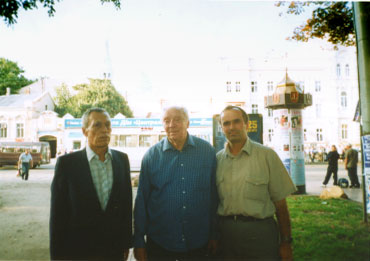
\includegraphics{photo}
  \end{center}
  \caption{V.G Vizing (L), A.A. Zykov (C), and V.I. Voloshin (R) in Odessa (2001) \cite{voloshin}}
\end{figure}

\subsubsection{The Chromatic Polynomial}

In his 1949 paper (translated by the AMS in 1952) \cite{zykov}, Zykov addresses the question: given a graph \(G\) and
a number \(k\in\N\), how many ways are there to properly color \(G\) using at most \(k\) colors?  In fact, he is not
particularly concerned about the chromatic number, which he calls the \emph{rank}, of a graph.  To solve this problem,
Zykov notes that in any proper coloring of a graph:
\begin{enumerate}
\item Nonadjacent vertices have either the same color or different colors.
\item Adjacent vertices always have different colors.
\end{enumerate}
If nonadjacent vertices have the same color then they can be contracted and the resulting graph retains the same
\coloring{k} as the original graph.  This is demonstrated in Figure \ref{fig:zvcon}.

\begin{figure}[h]
  \label{fig:zvcon}
  \begin{center}
    \begin{minipage}{2in}
      \begin{center}
        \begin{tikzpicture}[every node/.style={labeled node}]
          \colorlet{c1}{green!25!white}
          \colorlet{c2}{blue!25!white}
          \colorlet{c3}{red!25!white}
          \node (d) [fill=c2] at (0,0) {\(d\)};
          \node (c) [fill=c3,right=of d] {\(c\)};
          \node (b) [fill=c2,above=of c] {\(b\)};
          \node (a) [fill=c1,above=of d] {\(a\)};
          \draw (a) -- (b);
          \draw (a) -- (c) -- (d) -- (a);
        \end{tikzpicture}

        \bigskip

        \(G\)
      \end{center}
    \end{minipage}
    \begin{minipage}{2in}
      \begin{center}
        \begin{tikzpicture}[every node/.style={labeled node}]
          \colorlet{c1}{green!25!white}
          \colorlet{c2}{blue!25!white}
          \colorlet{c3}{red!25!white}
          \node (bd) [fill=c2] at (0,0) {\(bd\)};
          \node (c) [fill=c3,right=of bd] {\(c\)};
          \node (a) [fill=c1,above=of bd] {\(a\)};
          \draw (a) -- (c) -- (bd) -- (a);
        \end{tikzpicture}

        \bigskip

        \(G\cdot bd\)
      \end{center}
    \end{minipage}
  \end{center}
  \caption{Same Colors with Vertex Contraction}
\end{figure}

If nonadjacent vertices have different colors then they can be joined by an edge and the resulting graph retains
the same \coloring{k} as the original graph.  This is demonstrated in Figure \ref{fig:zeadd}.

\begin{figure}[h]
  \label{fig:zeadd}
  \begin{center}
    \begin{minipage}{2in}
      \begin{center}
        \begin{tikzpicture}[every node/.style={labeled node}]
          \colorlet{c1}{green!25!white}
          \colorlet{c2}{blue!25!white}
          \colorlet{c3}{red!25!white}
          \node (d) [fill=c2] at (0,0) {\(d\)};
          \node (c) [fill=c3,right=of d] {\(c\)};
          \node (b) [fill=c2,above=of c] {\(b\)};
          \node (a) [fill=c1,above=of d] {\(a\)};
          \draw (a) -- (b);
          \draw (a) -- (c) -- (d) -- (a);
        \end{tikzpicture}

        \bigskip

        \(G\)
      \end{center}
    \end{minipage}
    \begin{minipage}{2in}
      \begin{center}
        \begin{tikzpicture}[every node/.style={labeled node}]
          \colorlet{c1}{green!25!white}
          \colorlet{c2}{blue!25!white}
          \colorlet{c3}{red!25!white}
          \node (d) [fill=c2] at (0,0) {\(d\)};
          \node (c) [fill=c3,right=of d] {\(c\)};
          \node (b) [fill=c2,above=of c] {\(b\)};
          \node (a) [fill=c1,above=of d] {\(a\)};
          \draw (a) -- (b) -- (c);
          \draw (a) -- (c) -- (d) -- (a);
        \end{tikzpicture}

        \bigskip

        \(G+bc\)
      \end{center}
    \end{minipage}
  \end{center}
  \caption{Different Colors with Edge Addition}
\end{figure}

By applying these steps recursively, all of the possible distributions of the nonadjacent nodes to independent sets
are generated.  The termination condition for each recursive path is a complete graph of some varying order \(k\).
Each node in the complete graph represents an independent set of nonadjacent nodes in the original graph that have
been combined via vertex contraction.  Thus, each complete graph of order \(k\) represents a possible \coloring{k}
of the original graph.  The complete graphs of smallest order represent chromatic colorings and their order is the
chromatic number of the original graph.

Zykov uses a graph equation syntax to record the recursive processing of a graph, where each line in the equation
represents the next recursive layer.  Isomorphic graphs are combined with a frequency multiplier at each layer.
This is demonstrated in Figure \ref{fig:greqn}.

\begin{figure}[h]
  \label{fig:greqn}
  \begin{align*}
    \begin{minipage}{0.75in}
      \begin{center}
        \begin{tikzpicture}[every node/.style={unlabeled node}]
          \node (a1) at (0,0) {};
          \node (a2) [right=of a1] {};
          \node (a3) [above=of a2] {};
          \node (a4) [above=of a1] {};
          \draw (a3) -- (a4) -- (a1) -- (a2) -- (a4);
        \end{tikzpicture}
      \end{center}
    \end{minipage} &=
    \begin{minipage}{0.75in}
      \begin{center} 
        \begin{tikzpicture}[every node/.style={unlabeled node}]
          \node (b1) at (0,0) {};
          \node (b2) [above=of b1] {};
          \node (b3) [right=of b1] {};
          \draw (b1) -- (b2) -- (b3) -- (b1);
        \end{tikzpicture}
      \end{center}
    \end{minipage} +
    \begin{minipage}{0.75in}
      \begin{center}
        \begin{tikzpicture}[every node/.style={unlabeled node}]
          \node (c1) at (0,0) {};
          \node (c2) [right=of a1] {};
          \node (c3) [above=of a2] {};
          \node (c4) [above=of a1] {};
          \draw (c2) -- (c3) -- (c4) -- (c1) -- (c2) -- (c4);
        \end{tikzpicture}
      \end{center}
    \end{minipage} \\
    &= \begin{minipage}{0.75in}
      \begin{center} 
        \begin{tikzpicture}[every node/.style={unlabeled node}]
          \node (b1) at (0,0) {};
          \node (b2) [above=of b1] {};
          \node (b3) [right=of b1] {};
          \draw (b1) -- (b2) -- (b3) -- (b1);
        \end{tikzpicture}
      \end{center}
    \end{minipage} +
    \begin{minipage}{0.75in}
      \begin{center} 
        \begin{tikzpicture}[every node/.style={unlabeled node}]
          \node (b1) at (0,0) {};
          \node (b2) [above=of b1] {};
          \node (b3) [right=of b1] {};
          \draw (b1) -- (b2) -- (b3) -- (b1);
        \end{tikzpicture}
      \end{center}
    \end{minipage} +
    \begin{minipage}{0.75in}
      \begin{center}
        \begin{tikzpicture}[every node/.style={unlabeled node}]
          \node (c1) at (0,0) {};
          \node (c2) [right=of a1] {};
          \node (c3) [above=of a2] {};
          \node (c4) [above=of a1] {};
          \draw (c2) -- (c3) -- (c4) -- (c1) -- (c2) -- (c4);
          \draw (c1) -- (c3);
        \end{tikzpicture}
      \end{center}
    \end{minipage} \\
    &= 2
    \begin{minipage}{0.75in}
      \begin{center} 
        \begin{tikzpicture}[every node/.style={unlabeled node}]
          \node (b1) at (0,0) {};
          \node (b2) [above=of b1] {};
          \node (b3) [right=of b1] {};
          \draw (b1) -- (b2) -- (b3) -- (b1);
        \end{tikzpicture}
      \end{center}
    \end{minipage} +
    \begin{minipage}{0.75in}
      \begin{center}
        \begin{tikzpicture}[every node/.style={unlabeled node}]
          \node (c1) at (0,0) {};
          \node (c2) [right=of a1] {};
          \node (c3) [above=of a2] {};
          \node (c4) [above=of a1] {};
          \draw (c2) -- (c3) -- (c4) -- (c1) -- (c2) -- (c4);
          \draw (c1) -- (c3);
        \end{tikzpicture}
      \end{center}
    \end{minipage} \\
    &= 2K_3+K_4
  \end{align*}
  \caption{Zykov Graph Equation}
\end{figure}

Determining whether two graphs are isomorphic is hard, so combining isomorphic graphs in all but the very simple
cases should be skipped; the complete graphs resulting from the further processing of two isomorphic graphs will
eventually be combined anyway by the end.

Zykov was trying to determine the number of \coloring{k}s of a graph without color indifference: each permutation
of colors for a particular distribution is considered unique.  Thus, Zykov multiplied each complete graph
coefficient in the final line of a graph equation by the number of permutations from selecting the order \(n\) of
the particular complete graph from \(k\) colors:
\[k^{(n)}=k(k-1)(k-2)\cdots(k-n+1)\]
Thus, the total number of unique colorings from the example shown in Figure \ref{fig:greqn} using \(k\) colors
would be:
\[M(G,k)=2k^{(3)}+k^{(4)}\]
This is known as the factorial form of the \emph{chromatic polynomial} for the graph.  The corresponding
\emph{expanded form} is:
\[M(G,k)=k^4-4k^3+5k^2-2k\]
Read (1968) \cite{read} expands on the construction of the factorial form of the chromatic polynomial for a graph
and proves several theorems regarding the expanded form.  Some examples are:
\begin{enumerate}
\item \(M(G,k)=M(G\cdot uv)+M(G+uv)\), where \(u\) and \(v\) are any two nonadjacent vertices in the current
  recursive step.
\item The degree of M(G,k) is the order of \(G\).
\item The highest order coefficient is \(1\).
\item There is no constant term.
\item The terms alternate in sign.
\end{enumerate}
In fact, Read shows that the expanded form is actually an inclusion-exclusion equation resulting from starting with
all possible proper and improper colorings \(k^n\) and then subtracting the improper colorings.

\subsubsection{An Exhaustive Algorithm}

Corneil and Graham extend Zykov's work with the following theorem \cite{corneil}:

\begin{theorem}[Corneil and Graham, 1973]
  \label{thm:corneil}
  Let \(G\) be a graph and let \(u\) and \(v\) be two nonadjacent vertices in \(G\):
  \[\X(G)=\min\set{\X(G\cdot uv),\X(G+uv)}\]
\end{theorem}

Zykov's method combined with Theorem \ref{thm:corneil} can be used to construct an exhaustive algorithm for finding
the chromatic number and a chromatic coloring for a graph \(G\).  We define \(S\) to be a first-in-first out (FIFO)
stack of graphs and \(X\) to be the last found complete graph of the smallest order.  Each vertex in \(X\)
represents a set of contracted vertices.
\begin{enumerate}
\item Construct a graph \(G'\) that is isomorphic to \(G\) and where each vertex in \(G'\) is a list of contracted
  vertices initialized to a one element list containing the corresponding vertex in \(G\).
\item Push \(G'\) onto \(S\).
\item \label{step:zempty} If \(S\) is empty then return \(n(X)\) and \(X\).
\item \label{step:zcheck} If the graph on the top of \(S\) is complete:
  \begin{enumerate}
  \item Pop the graph off of the top of \(S\) and save it as \(H\).
  \item If \(X\) is not set or \(n(H)<n(X)\) then let \(X=H\).  Otherwise, discard \(H\).
  \item Go to step \ref{step:zempty}.
  \end{enumerate}
\item The graph on the top of \(S\) is not complete.  Pop the graph off of \(S\) and save it as \(H\).
\item Pick any two nonadjacent vertices \(u\) and \(v\) in \(H\).
\item Push \(H+uv\) onto \(S\).
\item Construct \(H'=H\cdot uv\), where the contracted vertex list for the new contracted vertex is a concatenation
  of the lists for \(u\) and \(v\).
\item Push \(H'\) onto \(S\).
\item Go to step \ref{step:zcheck}.
\end{enumerate}

The steps of this algorithm can be tracked via a so-called \emph{Zykov tree} \cite{corneil}.  The Zykov tree for
the example in Figure \ref{fig:greqn} is shown in Figure \ref{fig:ztree}.  Note that the exhaustive algorithm
corresponds to a depth-first walk of the tree.

\begin{figure}[h]
  \label{fig:ztree}
  \begin{center}
    \begin{tikzpicture}
      \node (a) [draw,circle] at (0,0) {
        \begin{tikzpicture}[every node/.style={unlabeled node}]
          \node (a1) at (0,0) {};
          \node (a2) [right=of a1] {};
          \node (a3) [above=of a2] {};
          \node (a4) [above=of a1] {};
          \draw (a3) -- (a4) -- (a1) -- (a2) -- (a4);
        \end{tikzpicture}
      };
      \node (b) [draw,circle,below left=of a] {
        \begin{tikzpicture}[every node/.style={unlabeled node}]
          \node (b1) at (0,0) {};
          \node (b2) [above=of b1] {};
          \node (b3) [right=of b1] {};
          \draw (b1) -- (b2) -- (b3) -- (b1);
        \end{tikzpicture}
      };
      \node (c) [draw,circle,below right=of a] {
        \begin{tikzpicture}[every node/.style={unlabeled node}]
          \node (c1) at (0,0) {};
          \node (c2) [right=of a1] {};
          \node (c3) [above=of a2] {};
          \node (c4) [above=of a1] {};
          \draw (c2) -- (c3) -- (c4) -- (c1) -- (c2) -- (c4);
        \end{tikzpicture}
      };
      \node (d) [draw,circle,below left=of c] {
        \begin{tikzpicture}[every node/.style={unlabeled node}]
          \node (d1) at (0,0) {};
          \node (d2) [above=of d1] {};
          \node (d3) [right=of d1] {};
          \draw (d1) -- (d2) -- (d3) -- (d1);
        \end{tikzpicture}
      };
      \node (e) [draw,circle,below right=of c] {
        \begin{tikzpicture}[every node/.style={unlabeled node}]
          \node (c1) at (0,0) {};
          \node (c2) [right=of a1] {};
          \node (c3) [above=of a2] {};
          \node (c4) [above=of a1] {};
          \draw (c2) -- (c3) -- (c4) -- (c1) -- (c2) -- (c4);
          \draw (c1) -- (c3);
        \end{tikzpicture}
      };
      \draw (a) edge (b) edge (c);
      \draw (c) edge (d) edge (e);
    \end{tikzpicture}
  \end{center}
  \caption{A Zykov Tree}
\end{figure}

\subsubsection{Branch and Bound Strategies}

Using a Zykov tree suggests that the exhaustive algorithm is a candidate for a branch-and-bound solution, where the
branching is accomplished via vertex contraction and edge addition and the bounding is some method to prematurely
terminate a branch.  Corneil and Graham suggest such a bounding technique through the determination of so-called
\(\a\)-clusters; however, the algorithm for finding such clusters has \(\BO(n^3)\) runtime complexity.


\section{The Proposed Algorithm}\label{sec:algorithm}

The major advantages of the Zykov and Christofides algorithms described in the previous section are that they don't
depend on the connectedness of a graph, an example of a chromatic coloring is readily available, and the fact that
the algorithms can be coded rather easily to run on a computer.  Their major disadvantage is its their high runtime
complexity, which as was shown is inherent to the chromatic number problem.

Thus, the goals of the proposed algorithm are as follows:
\begin{enumerate}
\item It should not depend on whether the graph is connected or not.
\item An example of a chromatic coloring should be available.
\item It can be easily coded for execution on a computer.
\item It has better runtime performance than the existing algorithms.
\end{enumerate}

To accomplish these goals, the proposed algorithm loops on successively higher values of \(k\).  For each candidate
\(k\) value, a graph is assumed to be \colorable{k} and a modified version of a Zykov algorithm is executed to
either prove or disprove this assumption.  Since a candidate \(k\) value is known, certain reversible steps can be
applied to mutate \(G\) into simpler graphs with equivalent colorability and test for early termination of the
current Zykov tree.  The first \(k\) for which \(G\) (or one of its simplifications) is found to be \colorable{k}
is the chromatic number of \(G\).

One slight disadvantage of the proposed algorithm is that whereas the other algorithms readily provide examples of
actual chromatic colorings, the proposed algorithm requires a reverse traversal of its reversible steps in order to
construct such a coloring.  However, as was stated earlier, it is more important during the axiomatic design
analytical process to know the minimum number of parts as opposed to an actual FR allocation to those parts.

This algorithm was first proposed by the author and his advisor in collaboration with a team of mechanical
engineering researchers from SUNY Buffalo \cite{cavallaro}.  It accepts a graph \(G\) as input, provides \(\X(G)\)
as output, and is composed of an outer loop on values of \(k\) and a subroutine called by the outer loop to
determine if \(G\) is \colorable{k}.  The outer loop and called subroutine are summarized in the following
sections.  A complete description of the theorems that support the various steps in algorithm and the application
of the algorithm to a sample graph then follow.

\subsection{Outer Loop}\label{sec:sub:outer}

The outer loop accepts a graph \(G\) as input and returns \(\X(G)\).  It initially checks for some degenerate cases
and then loops on increasing values of \(k\).  For each value of \(k\), the called subroutine executes a modified
Zykov algorithm to determine if \(G\) is \colorable{k}.  The first such successful return identifies \(\X(G)\).

The steps of the outer loop are as follows:

\begin{enumerate}
\item \label{step:outer:null} If \(n=0\) then return \(0\), thus handling the degenerate case of a null graph.

\item \label{step:outer:empty} If \(m=0\) then return \(1\), thus handling the degenerate case of an empty graph.

\item \label{step:outer:initk} Initialize \(k\) to \(2\).

\item \label{step:outer:call} Call the subroutine to determine if \(G\) is \colorable{k}.  The subroutine returns a
  possibly simplified \(G\) called \(G'\) and a boolean value \(R\) that reports the result of the test.

\item \label{step:outer:result} If \(G\) is \colorable{k} (\(R=\) true) then return \(k\).

\item \label{step:outer:newg} Replace \(G\) with \(G'\).  As will be seen, doing this avoids needless reapplication of
  certain steps in the called subroutine.

\item \label{step:outer:incrk} Increment \(k\).

\item \label{step:outer:loop} Go to step~\ref{step:outer:call}.
\end{enumerate}

A flowchart of these steps is shown in \figurename~\ref{fig:outer}.

\begin{figure}[H]
  \centering
  \scalebox{0.75}{
    \begin{tikzpicture}[>=latex']
      \node (start) [draw,terminal] at (0,0) {START};
      \node (nullcheck) [draw,decision,below=of start] {\(n=0\)?};
      \node (nulldone) [draw,terminal,right=of nullcheck] {RETURN \(0\)};
      \node (emptycheck) [draw,decision,below=of nullcheck] {\(m=0\)?};
      \node (emptydone) [draw,terminal,right=of emptycheck] {RETURN \(1\)};
      \node (kinit) [draw,process,below=of emptycheck] {\(k=2\)};
      \node (kcheck) [draw,predproc,below=of kinit] {CALL \(G,k\)};
      \node (iskcolor) [draw,decision,below=of kcheck] {\(R=\)TRUE?};
      \node (kdone) [draw,terminal,right=of iskcolor] {RETURN \(k\)};
      \node (newg) [draw,process,below=of iskcolor] {\(G=G'\)};
      \node (kinc) [draw,process,below=of newg] {\(k=k+1\)};
      \node (belowinc) [coordinate,below=0.5cm of kinc] {};
      \node (leftinc) [coordinate,left=3cm of belowinc] {};
      \draw [->] (start) -- node [auto] {\(G\)} (nullcheck);
      \draw [->] (nullcheck) -- node [auto] {YES} (nulldone);
      \draw [->] (nullcheck) -- node [auto] {NO} (emptycheck);
      \draw [->] (emptycheck) -- node [auto] {YES} (emptydone);
      \draw [->] (emptycheck) -- node [auto] {NO} (kinit);
      \draw [->] (kinit) -- (kcheck);
      \draw [->] (kcheck) -- node [auto] {\(G',R\)} (iskcolor);
      \draw [->] (iskcolor) -- node [auto] {YES} (kdone);
      \draw [->] (iskcolor) -- node [auto] {NO} (newg);
      \draw [->] (newg) -- (kinc);
      \draw [->] (kinc) -- (belowinc) -- (leftinc) |- (kcheck);
    \end{tikzpicture}
  }
  \caption{Proposed algorithm outer loop.}
  \label{fig:outer}
\end{figure}

The outer loop is guaranteed to terminate because \(k\) will eventually be greater than or equal to \(n\).  Thus,
by Proposition~\ref{prop:coloring3}, the current state of \(G\) is \colorable{k}, causing the called subroutine to
return true.

\subsection{Called Subroutine}\label{sec:sub:called}

The called subroutine executes a modified version of a Zykov algorithm that determines whether a graph is
\colorable{k}.  It accepts the current state of \(G\) of order \(n\) and size \(m\) and the current value of
\(k\ge2\) as inputs.  It returns a possibly simplified version of \(G\) and a boolean value indicating whether or
not \(G\) is \colorable{k}.  Internally, various tests are applied to trim the corresponding Zykov tree or abandon
it all together based on the current value of \(k\).

The steps of the called subroutine and references to their associated theorems are as follows:

\begin{enumerate}
\item \label{step:sub:check} If \(n\le k\) then return true (Proposition~\ref{prop:coloring3}).

\item \label{step:sub:dencalc} Calculate a maximum edge threshold:
  \[a=\frac{n^2(k-1)}{2k}\]

\item \label{step:sub:density} If \(m>a\) then return false (Corollary~\ref{cor:density}).

\item \label{step:sub:smallcalc} Construct the set \(X\) of all vertices with degree less than \(k\):
  \[X=\setb{v\in V(G)}{\deg(v)<k}\]

\item \label{step:sub:small} If \(X\ne\emptyset\) then replace \(G\) with \(G-X\) and go to
  step~\ref{step:sub:check} (Corollary~\ref{cor:lowdeg}).

\item \label{step:sub:common} Calculate the common number of neighbors between each pair of vertices in \(G\),
  stopping if one vertex's neighborhood is found to be a subset of another.

\item \label{step:sub:subset} If \(G\) has vertices \(u\) and \(v\) such that \(N(u)\subseteq N(v)\) then replace
  \(G\) with \(G-u\) and go to step~\ref{step:sub:check} (Theorem~\ref{thm:subset}).

\item \label{step:sub:select} Let \(b\) be the smallest number of common neighbors between any pair of vertices in
  \(G\) as found in step~\ref{step:sub:common}:
  \[b=\min_{u,v\in V(G)}\abs{N(u)\cap N(v)}\]

\item \label{step:sub:ubcalc} Calculate an upper bound for the minimum number of common neighbors between any pair of
  vertices in \(G\):
  \[c=n-2-\frac{n-2}{k-1}\]

\item \label{step:sub:ubcheck} If \(b>c\) then return false (Corollary~\ref{cor:inter}).

\item \label{step:sub:select2} Select two non-adjacent vertices \(u,v\in V(G)\) with the smallest number of common
  neighbors as found in step~\ref{step:sub:common}.  It will be shown below that such a pair of vertices is
  guaranteed to exist in the current state of \(G\).

\item \label{step:sub:call1} Assume that \(u\) and \(v\) are assigned the same color by letting \(G'=G\cdot uv\).
  Recursively call this routine to see if \(G'\) is \colorable{k}.  If so, then return true
  (Theorem~\ref{thm:recurse}).

\item \label{step:sub:call2} Assume that \(u\) and \(v\) are assigned different colors by letting \(G'=G+uv\).
  Recursively call this subroutine to see if \(G'\) is \colorable{k}.  If so, then return true
  (Theorem~\ref{thm:recurse}).

\item \label{step:sub:fail} Since neither of the assumptions in steps \ref{step:sub:call1} nor \ref{step:sub:call2}
  hold, conclude that \(G\) is not \colorable{k} and return false.
\end{enumerate}

A flowchart of these steps is shown in \figurename~\ref{fig:called}.

\begin{figure}[H]
  \centering
  \scalebox{0.65}{
    \begin{tikzpicture}[>=latex']
      \node (start) [draw,terminal] at (0,0) {START};
      \node (donecheck) [draw,decision,below=of start] {\(n\le k\)?};
      \node (done) [draw,terminal,right=of donecheck] {RETURN \(G\),TRUE};
      \node (edgecalc) [draw,process,below=of donecheck] {\(a=\frac{n^2(k-1)}{2k}\)};
      \node (edgecheck) [draw,decision,below=of edgecalc] {\(m>a\)?};
      \node (edgefail) [draw,terminal,right=of edgecheck] {RETURN \(G\),FALSE};
      \node (nodecalc) [draw,process,below=of edgecheck] {\(X=\setb{v\in V(G)}{\deg(v)<k}\)};
      \node (nodecheck) [draw,decision,below=of nodecalc] {\(X\ne\emptyset\)?};
      \node (remnode) [draw,process,left=of nodecheck] {\(G=G-X\)};
      \node (join) [coordinate] at ($(remnode)-(2.5cm,0)$) {};
      \node (common) [draw,process,below=of nodecheck] {Calculate \(\abs{N(u)\cap N(v)}\)};
      \node (subcheck) [draw,decision,below=of common] {\(N(u)\subseteq N(v)\)?};
      \node (remsub) [draw,process,left=of subcheck] {\(G=G-u\)};
      \node (mininter) [draw,process,below=of subcheck] {\(\displaystyle b=\min_{u,v\in V(G)}\abs{N(u)\cap N(v)}\)};
      \node (intercalc) [draw,process,below=of mininter] {\(c=n-2-\frac{n-2}{k-1}\)};
      \node (intercheck) [draw,decision,below=of intercalc] {\(b>c\)?};
      \node (interfail) [draw,terminal,right=of intercheck] {RETURN \(G\),FALSE};
      \node (finduv) [draw,process,right=2.5cm of done] {\(\displaystyle \min_{uv\notin E(G)}\abs{N(u)\cap N(v)}\)};
      \node (save1) [draw,process,below=of finduv] {\(G'=G\cdot uv\)};
      \node (call1) [draw,predproc,below=of save1] {CALL \(G',k\)};
      \node (check1) [draw,decision,below=of call1] {\(R=\)TRUE?};
      \node (done1) [draw,terminal,right=of check1] {RETURN \(G\),TRUE};
      \node (save2) [draw,process,below=of check1] {\(G'=G+uv\)};
      \node (call2) [draw,predproc,below=of save2] {CALL \(G',k\)};
      \node (check2) [draw,decision,below=of call2] {\(R=\)TRUE?};
      \node (done2) [draw,terminal,right=of check2] {RETURN \(G\),TRUE};
      \node (fail) [draw,terminal,below=of check2] {RETURN \(G\),FALSE};
      \draw [->] (start) -- node [auto] {\(G,k\)} (donecheck);
      \draw [->] (donecheck) -- node [auto] {YES} (done);
      \draw [->] (donecheck) -- node [auto] {NO} (edgecalc);
      \draw [->] (edgecalc) -- (edgecheck);
      \draw [->] (edgecheck) -- node [auto] {YES} (edgefail);
      \draw [->] (edgecheck) -- node [auto] {NO} (nodecalc);
      \draw [->] (nodecalc) -- (nodecheck);
      \draw [->] (nodecheck) -- node [auto] {YES} (remnode);
      \draw [->] (remnode) -- (join) |- (donecheck);
      \draw [->] (nodecheck) -- node [auto] {NO} (common);
      \draw [->] (common) -- (subcheck);
      \draw [->] (subcheck) -- node [auto] {YES} (remsub);
      \draw (remsub) -| (join);
      \draw [->] (subcheck) -- node [auto] {NO} (mininter);
      \draw [->] (mininter) -- (intercalc);
      \draw [->] (intercalc) -- (intercheck);
      \draw [->] (intercheck) -- node [auto] {YES} (interfail);
      \draw [->] (intercheck) -- node [auto] {NO} ($(intercheck)-(0,2cm)$) -- ++(7cm,0) |- (finduv);
      \draw [->] (finduv) -- (save1);
      \draw [->] (save1) -- (call1);
      \draw [->] (call1) -- node [auto] {\(G'',R\)} (check1);
      \draw [->] (check1) -- node [auto] {YES} (done1);
      \draw [->] (check1) -- node [auto] {NO} (save2);
      \draw [->] (save2) -- (call2);
      \draw [->] (call2) -- node [auto] {\(G'',R\)} (check2);
      \draw [->] (check2) -- node [auto] {YES} (done2);
      \draw [->] (check2) -- node [auto] {NO} (fail);
    \end{tikzpicture}
  }
  \caption{Proposed algorithm called subroutine.}
  \label{fig:called}
\end{figure}

Step~\ref{step:sub:check} is the success termination condition.  Success occurs when \(G\) is simplified by
removing sufficent vertices (steps~\ref{step:sub:smallcalc}--\ref{step:sub:subset}) or when the outer loop has
sufficiently incremented \(k\) (step~\ref{step:outer:incrk}) such that \(n\le k\).

Steps~\ref{step:sub:smallcalc}--\ref{step:sub:subset} attempt to remove vertices to achieve a simpler graph that is
equivalently \colorable{k}.  Each time a vertex is removed, the Zykov branches associated with that vertex are
skipped.  Since these same steps would just be repeated for \(k+1\), the subroutine returns the current state of
the possibly simplified \(G\) to the outer loop as a starting point for the next candidate value of \(k\).

Steps~\ref{step:sub:dencalc}--\ref{step:sub:density} and \ref{step:sub:select}--\ref{step:sub:ubcheck} apply tests
that attempt to disprove that the current state of \(G\) is \colorable{k} for the current value of \(k\).  If so,
then the current Zykov tree is abandoned and the subroutine returns false.  This allows the outer loop to continue
with \(k+1\).

The remaining steps of the called subroutine, steps~\ref{step:sub:select2}--\ref{step:sub:fail}, constitute the
recursive portion of the modified Zykov algorithm.  The recursive calls are guaranteed to terminate because either
there will be sufficient vertex contractions such that \(n\le k\), resulting in a true return, or sufficient edge
additions such that the graph becomes complete and (as will be shown) is rejected by step~\ref{step:sub:density},
resulting in a false return.  Note that in the event of a false return, any modifications to the current state of
\(G\) resulting from the recursive calls are not returned to the outer loop.

\subsection{Supporting Theorems}\label{sec:sub:theorems}

This section contains the theorems that support the steps in the called subroutine.  Remember that the success
check of step~\ref{step:sub:check} is already supported by Proposition~\ref{prop:coloring3}.

\subsubsection{Maximum Edge Threshold}\label{sec:sub:sub:edges}

The maximum edge threshold test of steps~\ref{step:sub:dencalc} and \ref{step:sub:density} is supported by
Theorem~\ref{thm:density}.

\begin{theorem}[Maximum Edge Threshold]
  \label{thm:density}
  Let \(G\) be a graph of order \(n\) and size \(m\) and let \(k\in\N\).  If \(G\) is \colorable{k} then:
  \[m\le\frac{n^2(k-1)}{2k}\]
\end{theorem}

\begin{proof}
  Assume that \(G\) is \colorable{k}.  This means that \(V(G)\) can be distributed into \(k\) independent (some
  possibly empty) subsets.  Call these subsets \(A_1,\ldots A_k\) and let \(a_i=\abs*{A_i}\).  Thus, each \(v\in
  A_i\) can be adjacent to at most \(n-a_i\) other vertices in \(G\), and hence the maximum number of edges
  incident to vertices in \(A_i\) is given by: \(a_i(n-a_i)=na_i-a_i^2\).  Now, using Theorem~\ref{thm:first}, the
  maximum number of edges in \(G\) is given by:
  \[m\le\frac{1}{2}\sum_{i=1}^k(na_i-a_i^2)\]
  with the constraint:
  \[\sum_{i=1}^ka_i=n\]
  This problem can be solved using the Lagrange multiplier technique.  We start by defining:
  \begin{align*}
    F(a_1,\ldots,a_k) &= f(a_1,\ldots,a_k)-\l g(a_1,\ldots,a_k) \\
    &= \frac{1}{2}\sum_{i=1}^k(na_i-a_i^2)-\l\sum_{i=1}^ka_i \\
    &= \sum_{i=1}^k\left(\frac{1}{2}na_i-\frac{1}{2}a_i^2-\l a_i\right)
  \end{align*}
  Now, optimize by taking the gradient and setting the resulting vector equation equal to the zero vector:
  \[\vec{\nabla}F=\sum_{i=1}^k(\frac{n}{2}-a_i-\l)\hat{a_i}=\vec{0}\]
  This results in a system of \(k\) equations of the form:
  \[\frac{n}{2}-a_i-\l=0\]
  And so:
  \[a_i=\frac{n}{2}-\l\]
  Plugging this result back into the contraint:
  \[\sum_{i=1}^ka_i=\sum_{i=1}^k\left(\frac{n}{2}-\l\right)=k\left(\frac{n}{2}-\l\right)=n\]
  Solving for \(\l\) yields:
  \[\l=\frac{n}{2}-\frac{n}{k}\]
  And finally, to get \(a_i\) in terms of \(n\) and \(k\):
  \[a_i=\frac{n}{2}-\left(\frac{n}{2}-\frac{n}{k}\right)=\frac{n}{k}\]
  Therefore:
  \[m\le\frac{1}{2}\sum_{i=1}^k\left[n\left(\frac{n}{k}\right)-\left(\frac{n}{k}\right)^2\right]=
  \frac{k}{2}\left(\frac{n^2k-n^2}{k^2}\right)=\frac{n^2(k-1)}{2k}\]
\end{proof}

The called subroutine actually uses the contrapositive of this result, as stated in Corollary~\ref{cor:density}.

\begin{corollary}
  \label{cor:density}
  Let \(G\) be a graph of order \(n\) and size \(m\) and let \(k\in\N\).  If:
  \[m>\frac{n^2(k-1)}{2k}\]
  then \(G\) is not \colorable{k}.
\end{corollary}

Corollary~\ref{cor:density} is demonstrated by \figurename~\ref{fig:density}.  The shown graph \(G\) has \(n=4\),
\(m=5\), and \(\X(G)=3\).  Testing for \(k=2\):
\[a=\frac{4^2(2-1)}{2\cdot2}=4\]
But \(m=5>4=a\) and so we can conclude that \(G\) is not \colorable{2}.  However, testing for \(k=3\);
\[a=\frac{4^2(3-1)}{2\cdot3}=5.3\]
So \(m=5\ngtr5.3=a\) and thus \(G\) \emph{may} be \(3\)-colorable, since this test only provides a necessary and
not a sufficient condition.

\begin{figure}[H]
  \centering
  \begin{tikzpicture}
    \colorlet{c1}{green!25!white}
    \colorlet{c2}{blue!25!white}
    \colorlet{c3}{red!25!white}
    \begin{scope}[every node/.style={coordinate}]
      \cycleNnodes{4}{(0,0)}{0.75in}{135}{c};
    \end{scope}
    \begin{scope}[every node/.style={labeled node}]
      \node [fill=c1] (a) at (c1) {\(a\)};
      \node [fill=c2] (b) at (c2) {\(b\)};
      \node [fill=c1] (c) at (c3) {\(c\)};
      \node [fill=c3] (d) at (c4) {\(d\)};
    \end{scope}
    \draw (a) edge (b) edge (d);
    \draw (b) edge (c) edge (d);
    \draw (c) edge (d);
  \end{tikzpicture}

  \(G\)
  \caption{Corollary~\ref{cor:density} example.}
  \label{fig:density}
\end{figure}

In fact, the the test of Corollary~\ref{cor:density} will always fail for a complete graph when \(k<n\).  Since
\(k,n>0\):
\begin{align*}
  \frac{n(n-1)}{2}-\frac{n^2(k-1)}{2k} &= \frac{kn(n-1)-n^2(k-1)}{2k} \\
  &= \frac{kn^2-kn-kn^2+n^2}{2k} \\
  &= \frac{n^2-kn}{2k} \\
  &= \frac{n(n-k)}{2k} \\
  &>0\qquad(n>k)
\end{align*}

\subsubsection{Vertex Removal}\label{sec:sub:sub:vremove}

The theorems that support vertex removal make use of Lemma~\ref{lem:remone}.

\begin{lemma}
  \label{lem:remone}
  Let \(G\) be a graph and let \(v\in V(G)\).  If \(G\) is \colorable{k} then \(G-v\) is also \colorable{k}.
\end{lemma}

\begin{proof}
  Assume that \(G\) is \colorable{k}.  Let \(c:V(G)\to C\) be such a coloring, and so \(\abs{C}=k\).  Intuitively,
  removing \(v\) from \(G\) should not affect the proper coloring of the remaining vertices.  Thus, we should be
  able to construct a proper coloring for \(G-v\) based upon \(c\).  So consider the restricted coloring function
  \(c'=\restrict{c}{V(G-v)}\) and assume \(uw\in E(G-v)\).  Since \(c\) is proper:
  \[c'(u)=c(u)\ne c(w)=c'(w)\]
  Thus, \(c'\) is a proper coloring of \(G-v\) using at most \(k\) colors.

  Therefore \(G-v\) is \colorable{k}.
\end{proof}

Lemma~\ref{lem:remone} is demonstrated in \figurename~\ref{fig:remone}.  No matter which vertex is removed, the
resulting subgraph is still properly colored using at most four (in fact, three) colors.

\begin{figure}[H]
  \centering
  \scalebox{0.75}{
    \begin{tikzpicture}
      \colorlet{c1}{green!25!white}
      \colorlet{c2}{blue!25!white}
      \colorlet{c3}{red!25!white}
      \colorlet{c4}{yellow!25!white}
      \begin{scope}[every node/.style={coordinate}]
        \cycleNnodes{4}{(0,0)}{0.5in}{135}{x};
      \end{scope}
      \begin{scope} [every node/.style={labeled node}]
        \node [fill=c1] (v1) at (x1) {\(a\)};
        \node [fill=c2] (v2) at (x2) {\(b\)};
        \node [fill=c3] (v3) at (x3) {\(c\)};
        \node [fill=c4] (v4) at (x4) {\(d\)};
      \end{scope}
      \draw (v1) edge (v2) edge (v3) edge (v4);
      \draw (v2) edge (v3) edge (v4);
      \draw (v3) edge (v4);
    \end{tikzpicture}
  }

  \(G\)

  \bigskip

  \begin{minipage}{1.25in}
    \centering
    \scalebox{0.75}{
      \begin{tikzpicture}
        \colorlet{c1}{green!25!white}
        \colorlet{c2}{blue!25!white}
        \colorlet{c3}{red!25!white}
        \colorlet{c4}{yellow!25!white}
        \begin{scope}[every node/.style={coordinate}]
          \cycleNnodes{4}{(0,0)}{0.5in}{135}{x};
        \end{scope}
        \begin{scope} [every node/.style={labeled node}]
          \node [fill=c2] (v2) at (x2) {\(b\)};
          \node [fill=c3] (v3) at (x3) {\(c\)};
          \node [fill=c4] (v4) at (x4) {\(d\)};
        \end{scope}
        \draw (v2) edge (v3) edge (v4);
        \draw (v3) edge (v4);
      \end{tikzpicture}
    }

    \(G-a\)
  \end{minipage}
  \begin{minipage}{1.25in}
    \centering
    \scalebox{0.75}{
      \begin{tikzpicture}
        \colorlet{c1}{green!25!white}
        \colorlet{c2}{blue!25!white}
        \colorlet{c3}{red!25!white}
        \colorlet{c4}{yellow!25!white}
        \begin{scope}[every node/.style={coordinate}]
          \cycleNnodes{4}{(0,0)}{0.5in}{135}{x};
        \end{scope}
        \begin{scope} [every node/.style={labeled node}]
          \node [fill=c1] (v1) at (x1) {\(a\)};
          \node [fill=c3] (v3) at (x3) {\(c\)};
          \node [fill=c4] (v4) at (x4) {\(d\)};
        \end{scope}
        \draw (v1) edge (v3) edge (v4);
        \draw (v3) edge (v4);
      \end{tikzpicture}
    }

    \(G-b\)
  \end{minipage}
  \begin{minipage}{1.25in}
    \centering
    \scalebox{0.75}{
      \begin{tikzpicture}
        \colorlet{c1}{green!25!white}
        \colorlet{c2}{blue!25!white}
        \colorlet{c3}{red!25!white}
        \colorlet{c4}{yellow!25!white}
        \begin{scope}[every node/.style={coordinate}]
          \cycleNnodes{4}{(0,0)}{0.5in}{135}{x};
        \end{scope}
        \begin{scope} [every node/.style={labeled node}]
          \node [fill=c1] (v1) at (x1) {\(a\)};
          \node [fill=c2] (v2) at (x2) {\(b\)};
          \node [fill=c4] (v4) at (x4) {\(d\)};
        \end{scope}
        \draw (v1) edge (v2) edge (v4);
        \draw (v2) edge (v4);
      \end{tikzpicture}
    }

    \(G-c\)
  \end{minipage}
  \begin{minipage}{1.25in}
    \centering
    \scalebox{0.75}{
      \begin{tikzpicture}
        \colorlet{c1}{green!25!white}
        \colorlet{c2}{blue!25!white}
        \colorlet{c3}{red!25!white}
        \colorlet{c4}{yellow!25!white}
        \begin{scope}[every node/.style={coordinate}]
          \cycleNnodes{4}{(0,0)}{0.5in}{135}{x};
        \end{scope}
        \begin{scope} [every node/.style={labeled node}]
          \node [fill=c1] (v1) at (x1) {\(a\)};
          \node [fill=c2] (v2) at (x2) {\(b\)};
          \node [fill=c3] (v3) at (x3) {\(c\)};
        \end{scope}
        \draw (v1) edge (v2) edge (v3);
        \draw (v2) edge (v3);
      \end{tikzpicture}
    }

    \(G-d\)
  \end{minipage}
  \caption{Lemma~\ref{lem:remone} example.}
  \label{fig:remone}
\end{figure}

Steps~\ref{step:sub:smallcalc} and \ref{step:sub:small} remove vertices with degrees less than \(k\).  This is
supported by Theorem~\ref{thm:lowdeg}.

\begin{theorem}
  \label{thm:lowdeg}
  Let \(G\) be a graph and let \(v\in V(G)\) such that \(\deg(v)<k\) for some \(k\in\N\).  \(G\) is \colorable{k}
  if and only if \(G-v\) is \colorable{k}.
\end{theorem}

\begin{proof}
  Assume that \(G\) is \colorable{k}.  Therefore, by Lemma~\ref{lem:remone}, \(G-v\) is also \colorable{k}.

  For the converse, assume that \(G-v\) is \colorable{k}.  Let \(c:V(G-v)\to C\) be such a coloring, and so
  \(\abs{C}=k\).  By assumption, \(\deg(v)<k\), so \(v\) has at most \(k-1\) neighbors in \(G\), using at most
  \(k-1\) colors.  This means that there should be an additional color that can be assigned to \(v\) in \(G\) such
  that the coloring remains proper.  So let \(N(v)=\set{v_1,\ldots,v_r}\subseteq V(G-v)\) for some \(r<k\), and let
  \(c[N(v)]=\set{c_1,\ldots,c_s}\subset C\) for some \(s\le r<k\).  Since \(c[N(v)]\) is a proper subset of \(C\),
  select \(c_k\in C-c[N(v)]\) and define \(c':V(G)\to C\) as follows:
  \[c'(u)=\begin{cases}
  c(u), & u\ne v \\
  c_k, & u=v
  \end{cases}\]
  Now, assume that \(uw\in E(G)\) and consider the following two cases:
  \begin{description}
  \item[Case 1:] \(v\notin uw\)

    Since \(c\) is proper:
    \[c'(u)=c(u)\ne c(w)=c'(w)\]
  \item[Case 2:] \(v\in uw\)

    Assume without loss of generality (AWLOG) that \(u=v\).  This means that \(c'(v)=c_k\) and \(c'(w)=c(w)\in
    c[N(v)]\).  But \(c_k\notin c[N(v)]\) and so \(c'(v)\ne c'(w)\).
  \end{description}
  Thus, \(c'\) is a proper coloring of \(G\) using at most \(k\) colors.

  Therefore \(G\) is \colorable{k}.
\end{proof}

Theorem~\ref{thm:lowdeg} is demonstrated in \figurename~\ref{fig:lowdeg} for \(k=4\) and \(\deg(v)=3\).

\begin{figure}[H]
  \centering
  \begin{tikzpicture}
    \colorlet{c1}{green!25!white}
    \colorlet{c2}{blue!25!white}
    \colorlet{c3}{red!25!white}
    \colorlet{c4}{yellow!25!white}
    \begin{scope}[every node/.style={coordinate}]
      \cycleNnodes{4}{(0,0)}{1in}{135}{c};
    \end{scope}
    \begin{scope}[every node/.style={labeled node}]
      \node [fill=c1] (a) at (c1) {\(a\)};
      \node [fill=c2] (v) at (c2) {\(v\)};
      \node [fill=c3] (b) at (c3) {\(b\)};
      \node [fill=c4] (c) at (c4) {\(c\)};
      \node [fill=c2,below left=of a] (d) {\(d\)};
    \end{scope}
    \draw (a) edge (b) edge (c) edge (d);
    \draw [dashed,red] (v) edge (a) edge (b) edge (c);
    \draw (b) edge (c);
    \draw (c) edge (d);
  \end{tikzpicture}
  \caption{Theorem~\ref{thm:lowdeg} example.}
  \label{fig:lowdeg}
\end{figure}

The called subroutine actually removes all such vertices at once, which is supported by the inductive proof in
Corollary \ref{cor:lowdeg}.

\begin{corollary}
  \label{cor:lowdeg}
  Let \(G\) be a graph of order \(n\) and let \(X=\setb{v\in V(G)}{\deg(v)<k}\) for some \(k\in\N\).  \(G\) is
  \colorable{k} if and only if \(G-X\) is \colorable{k}.
\end{corollary}

\begin{proof}
  (by induction on \(\abs{X}\))
  \begin{description}
  \item[Base Case:] Let \(\abs{X}=0\).

    But \(G-X=G\) (trivial case).

  \item[Inductive Assumption:] Let \(\abs{X}=r\).

    Assume that \(G\) is \colorable{k} if and only if \(G-X\) is \colorable{k}.

  \item[Inductive Step:] Consider \(\abs{X}=r+1\).
    
    Since \(\abs{X}=r+1>0\), there exists \(v\in X\) such that \(\deg(v)<k\).  Let \(Y=X-\set{v}\) and note that
    \(\abs{Y}=\abs{X}-1=(r+1)-1=r\).  So, \(G\) is \colorable{k} if and only if \(G-v\) is \colorable{k} (Theorem
    \ref{thm:lowdeg}) if and only if \((G-v)-Y\) is \colorable{k} (inductive assumption).
  \end{description}

  Therefore, by the principle of induction, \(G\) is \colorable{k} if and only if \(G-X\) is \colorable{k}.
\end{proof}

Returning to the example in \figurename~\ref{fig:lowdeg}, note that \(X=\set{v,b}\) is the set of all vertices with
degree less than \(4\) and so both could be removed at once in accordance with Corollary \ref{cor:lowdeg}.
Furthermore, after these vertices are removed, the remaining vertices \(a\), \(b\), and \(c\) will all have degree
\(2\).  Since \(2<4\), the remaining vertices are subsequently removed, leaving \(n=0<4\), indicating that the
graph is indeed \colorable{4}.  This iterative collapsing of a graph is an ideal situation.

Step~\ref{step:sub:subset} removes vertices whose neighborhoods are subsets of other vertices.  This is supported
by Theorem~\ref{thm:subset}.

\begin{theorem}
  \label{thm:subset}
  Let \(G\) be a graph and let \(u,v\in V(G)\) such that \(N(u)\subseteq N(v)\).  \(G\) is \colorable{k} if and
  only if \(G-u\) is \colorable{k}.
\end{theorem}

\begin{proof}
  Assume that \(G\) is \colorable{k}.  Therefore, by Lemma \ref{lem:remone}, \(G-u\) is also \colorable{k}.

  For the converse, assume that \(G-u\) is \colorable{k}.  Let \(c:V(G-u)\to C\) be such a coloring, and so
  \(\abs{C}=k\).  By definition, \(u\notin N(u)\), and since, by assumption, \(N(u)\subseteq N(v)\), it is also the
  case that \(u\notin N(v)\).  Hence, \(u\) is not adjacent to \(v\) in \(G\).  But everything that is adjacent to
  \(u\) in \(G\) is also adjacent to \(v\) in both \(G-u\) and \(G\).  Since everything adjacent to \(v\) has a
  different color than \(v\), we should be able to assign \(u\) the same color as \(v\) in \(G\) in order to get a
  proper coloring of \(G\).

  Let \(S=N(u)\cap N(v)=\set{w_1,\ldots w_r}\subset V(G-u)\) for some \(r=\deg(u)\le \deg(v)\).  For all \(w\in
  S\), \(w\in N(v)\) meaning \(vw\in E(G-u)\).  And, because \(c\) is proper, it must be the case that \(c(w)\ne
  c(v)\).  So define \(c':V(G)\to C\) as follows:
  \[c'(w)=\begin{cases}
  c(w), & w\ne u \\
  c(v), & w=u
  \end{cases}\]
  Now, assume that \(wz\in E(G)\) and consider the following two cases:
  \begin{description}
  \item[Case 1:] \(u\notin wz\)

    Since \(c\) is proper:
    \[c'(w)=c(w)\ne c(z)=c'(z)\]
  \item[Case 2:] \(u\in wz\)

    Assume without loss of generality (AWLOG) that \(u=w\).  Since \(vz\in E(G)\) and \(c\) is proper:
    \[c'(u)=c(v)\ne c(z)=c'(z)\]
  \end{description}
  Thus, \(c'\) is a proper coloring of \(G\) using at most \(k\) colors.

  Therefore \(G\) is \colorable{k}.
\end{proof}

Theorem~\ref{thm:subset} is demonstrated in \figurename~\ref{fig:subset}.  Since \(N(u)\subseteq N(v)\), \(G\) and
\(G-u\) are equivalently colorable.  Futhermore, once \(u\) is removed, the degrees of vertices \(a\) and \(c\)
will have degree \(2\).  So if \(k=3\), those two vertices are subsequently removed by step \ref{step:sub:small}.
The remaining graph is of order \(2\), which then passes the success check of step \ref{step:sub:check} because
\(2<3\), so indeed the graph is \colorable{3}.  Once again, this iterative removal of vertices is very powerful.

\begin{figure}[H]
  \centering
  \begin{tikzpicture}[every node/.style={labeled node}]
    \colorlet{c1}{green!25!white}
    \colorlet{c2}{blue!25!white}
    \colorlet{c3}{red!25!white}
    \node [fill=c1] (b) at (0,0) {\(b\)};
    \node [fill=c2] (a) [above=of b] {\(a\)};
    \node [fill=c2] (c) [below=of b] {\(c\)};
    \node [fill=c3] (u) [left=of b] {\(u\)};
    \node [fill=c3] (v) [right=of b] {\(v\)};
    \draw [dashed,red] (u) edge (a) edge (b);
    \draw (v) edge (a) edge (b) edge (c);
    \draw (a) edge (b);
    \draw (c) edge (b);
  \end{tikzpicture}
  \caption{Theorem \ref{thm:subset} example.}
  \label{fig:subset}
\end{figure}

\subsubsection{Minimum Common Neighbor Upper Bound}\label{sec:sub:sub:common}

Steps~\ref{step:sub:select}--\ref{step:sub:ubcheck} establish an upper bound for the minimum common neighbor count
between any two vertices in a graph that is assumed to be \colorable{k}.  This limit is dependent on the following
facts that are guaranteed by previous steps:

\begin{enumerate}
\item \(2\le k<n\)
\item There are no \(u,v\in V(G)\) such that \(N(u)\subseteq N(v)\)
\end{enumerate}

The supporting theorem uses these facts along with Lemma~\ref{lem:neighbor} in its proof.

\begin{lemma}
  \label{lem:neighbor}
  Let \(G\) be a graph and let \(S\) be a non-empty independent subset of \(V(G)\).  If there exists a vertex
  \(v\in S\) such that \(v\) is adjacent to all vertices in \(V(G)-S\) (i.e., \(N(v)=V(G)-S\)) then for all
  vertices \(u\in S\) it is the case that \(N(u)\subseteq N(v)\).
\end{lemma}

\begin{proof}
  Assume that such a \(v\) exists and then assume that \(u\in S\).  If \(u=v\) then (trivially) \(N(v)=N(v)\), so
  assume \(u\ne v\).  Furthermore, since \(u,v\in S\) and \(S\) is independent (by assumption), it must be the case
  that \(u\) and \(v\) are not neighbors.

  \begin{description}
  \item[Case 1:] \(N(u)=\emptyset\).
      
    Therefore, by definition, \(N(u)=\emptyset\subseteq N(v)\).

  \item[Case 2:] \(N(u)\ne\emptyset\).

    Assume that \(w\in N(u)\).  This means that \(w\) is adjacent to \(u\) and hence \(w\notin S\), since \(S\) is
    an independent set.  So \(w\in V(G)-S\) and thus, by assumption, \(v\) is adjacent to \(w\) and we can conclude
    that \(w\in N(v)\).  Therefore \(N(u)\subseteq N(v)\).
  \end{description}

  Therefore, for all \(u\in S\), \(N(u)\subseteq N(v)\).
\end{proof}

Lemma~\ref{lem:neighbor} is demonstrated in \figurename~\ref{fig:neighbor}.  Note that since \(v\in S\) is adjacent
to every vertex in \(V(G)-S\), vertex \(u\in S\) can't help but be adjacent to some subset of \(N(v)\).

\begin{figure}[H]
  \centering
  \begin{tikzpicture}
    \draw (0in,0) ellipse (0.5in and 1in);
    \draw (3in,0) ellipse (1.5in and 1in);
    \begin{scope}[every node/.style={unlabeled node}]
      \node (v) at (0in,0.25in) {};
      \node (u) at (0in,-0.25in) {};
      \node (w1) at (2in,0) {};
      \node (w2) at (2.5in,0) {};
      \node (w3) at (3in,0) {};
      \node (w4) at (3.5in,0) {};
      \node (w5) at (4in,0) {};
    \end{scope}
    \node [left=1ex of v] {\(v\)};
    \node [left=1ex of u] {\(u\)};
    \node at (0,-1.25in) {\(S\)};
    \node at (3in,-1.25in) {\(V(G)-S\)};
    \draw (v) [bend left] edge (w1);
    \draw (v) [bend left] edge (w2);
    \draw (v) [bend left] edge (w3);
    \draw (v) [bend left] edge (w4);
    \draw (v) [bend left] edge (w5);
    \draw (u) [bend right] edge (w2);
    \draw (u) [bend right] edge (w4);
    \draw (u) [bend right] edge (w5);
  \end{tikzpicture}
  \caption{Lemma \ref{lem:neighbor} example.}
  \label{fig:neighbor}
\end{figure}

Theorem~\ref{thm:inter} establishes the desired upper bound.

\begin{theorem}
  \label{thm:inter}
  Let \(G\) be a graph of order \(n\) and size \(m\) such that there are no \(u,v\in V(G)\) where \(N(u)\subseteq
  N(v)\), and let \(k\in\N\) such that \(2\le k<n\).  If \(G\) is \colorable{k} then there exists two vertices
  \(w,z\in V(G)\) such that:
  \[\abs{N(w)\cap N(z)}\le n-2-\frac{n-2}{k-1}\]
\end{theorem}

\begin{proof}
  Assume that \(G\) is \colorable{k}.  This means that \(V(G)\) can be distributed into \(k\) independent (some
  possibly empty) subsets \(A_1,\ldots,A_k\) such that \(a_i=\abs*{A_i}\) and \(a_1\ge a_2\ge\cdots\ge a_k\).
  Since \(n>k\), by the pigeonhole principle, it must be the case that \(a_1\ge2\).  Assume that \(v\in A_1\).

  First, assume by way of contradiction (ABC) that \(v\) is adjacent to all other vertices in \(V(G)-A_1\).  Since
  \(a_1\ge2\), there exists \(u\in A_1\) such that \(u\ne v\) and \(u\) is not adjacent to \(v\).  Thus, by Lemma
  \ref{lem:neighbor}, \(N(u)\subseteq N(v)\), contradicting the assumption.  Note that this contradiction also
  eliminates the degenerate case where \(A_1=V(G)\); however, this case does not occur here because the graph would
  be an empty graph and would have been eliminated by previous steps.  Therefore, there exists some \(v'\in
  V(G)-A_1\) such that \(v\) is not adjacent to \(v'\).  Assume that \(v'\in A_i\) for some \(i\) such that
  \(1<i\le k\):

  \begin{description}
  \item [Case 1:] \(a_i=1\)

    By the pigeonhole principle:
    \[a_1\ge\ceil*{\frac{n-1}{k-1}}\ge\frac{n-1}{k-1}\]
    Now, assume by way of contradiction (ABC) that \(v'\) is adjacent to all vertices in \(V(G)-A_1-A_i\) and
    assume \(u\in N(v)\).  Then it must be the case that \(u\in V(G)-A_1-A_i\), and so \(u\) is adjacent to \(v'\),
    and thus \(u\in N(v')\).  Therefore \(N(v)\subseteq N(v')\), which contradicts the assumption.  This situation
    is demonstrated by \figurename~\ref{fig:aione}.

    \begin{figure}[H]
      \centering
      \begin{tikzpicture}
        \draw (0,0) ellipse (0.5in and 1in);
        \draw (2in,0) ellipse (0.5in and 1in);
        \draw (4in,0) ellipse (0.5in and 1in);
        \begin{scope}[every node/.style={unlabeled node}]
          \node (v) at (0,0) {};
          \node (u1) at (2in,0.5in) {};
          \node (u2) at (2in,0.25in) {};
          \node (u3) at (2in,0in) {};
          \node (u4) at (2in,-0.25in) {};
          \node (u5) at (2in,-0.5in) {};
          \node (vp) at (4in,0) {};
        \end{scope}
        \node [left=1ex of v] {\(v\)};
        \node [right=1ex of vp] {\(v'\)};
        \node at (0,-1.25in) {\(A_1\)};
        \node at (2in,-1.25in) {\(V(G)-A_1-A_i\)};
        \node at (4in,-1.25in) {\(A_i\)};
        \draw (v) edge (u1) edge (u3) edge (u4);
        \draw (vp) edge (u1) edge (u2) edge (u3) edge (u4) edge (u5);
      \end{tikzpicture}
      \caption{Case \(a_i=1\) contradiction.}
      \label{fig:aione}
    \end{figure}

    So there must exist some \(u\in V(G)-A_1-A_i\) such that \(u\) is not adjacent to \(v'\).  This results in the
    upper bound:
    \[\abs{N(v)\cap N(v')}\le n-\abs{\set{u,v'}}-a_1\le n-2-\frac{n-1}{k-1}\]
    Note that since \(v\in A_1\), it is already counted in \(a_1\).  Comparing this bound to the desired bound:
    \[\left(n-2-\frac{n-2}{k-1}\right)-\left(n-2-\frac{n-1}{k-1}\right)=\frac{(n-1)-(n-2)}{k-1}=\frac{1}{k-1}>0\]
    for \(k\ge2\).  Thus the new bound is tighter and so:
    \[\abs{N(v)\cap N(v')}\le n-2-\frac{n-1}{k-1}\le n-2-\frac{n-2}{k-1}\]
    
  \item [Case 2:] \(a_i=2\)

    By the pigeonhole principle:
    \[a_1\ge\ceil*{\frac{n-2}{k-1}}\ge\frac{n-2}{k-1}\]
    This results in the upper bound:
    \[\abs{N(v)\cap N(v')}\le n-a_i-a_1\le n-2-\frac{n-2}{k-1}\]
    
  \item [Case 3:] \(a_i\ge3\)

    By the pigeonhole principle:
    \[a_1\ge\ceil*{\frac{n-3}{k-1}}\ge\frac{n-3}{k-1}\]
    This results in the upper bound:
    \[\abs{N(v)\cap N(v')}\le n-a_i-a_1\le n-3-\frac{n-3}{k-1}\]
    Comparing this to the desired bound:
    \[\left(n-2-\frac{n-2}{k-1}\right)-\left(n-3-\frac{n-3}{k-1}\right)=1-\frac{(n-3)-(n-2)}{k-1}=1-\frac{1}{k-1}>0\]
    for \(k\ge2\).  Thus the new bound is tighter and so:
    \[\abs{N(v)\cap N(v')}\le n-3-\frac{n-3}{k-1}\le n-2-\frac{n-2}{k-1}\]
  \end{description}

  Therefore, there exists \(w,v\in V(G)\) such that:
  \[\abs{N(w)\cap N(z)}\le n-2-\frac{n-2}{k-1}\]
\end{proof}

The called subroutine actually uses the contrapositive of this result, as stated in Corollary~\ref{cor:inter}.

\begin{corollary}
  \label{cor:inter}
  Let \(G\) be a graph of order \(n\) and size \(m\) such that there are no \(u,v\in V(G)\) where
  \(N(u)\subseteq N(v)\), and let \(k\in\N\) such that \(2\le k<n\).  If for all \(w,z\in V(G)\) it is the case
  that:
  \[\abs{N(w)\cap N(z)}>n-2-\frac{n-2}{k-1}\]
  then \(G\) is not \colorable{k}.
\end{corollary}

Corollary~\ref{cor:inter} is demonstrated in \figurename~\ref{fig:inter}.  The shown graph has \(n=5\), is
\chromatic{3}, and has:
\[\min_{u,v\in V(G)}\abs{N(u)\cap N(v)}=1\]
Testing for \(k=2\):
\[5-2-\frac{5-2}{2-1}=0\]
But \(1>0\) and so we can conclude that \(G\) is not \colorable{2}.  However, testing for \(k=3\):
\[5-2-\frac{5-2}{3-1}=\frac{3}{2}\]
So \(1\ngtr\frac{3}{2}\) and thus \(G\) \emph{may} be \colorable{3}, since this test only provides a necessary and
not a sufficient condition.

\begin{figure}[H]
  \centering
  \begin{tikzpicture}
    \colorlet{c1}{green!25!white}
    \colorlet{c2}{blue!25!white}
    \colorlet{c3}{red!25!white}
    \begin{scope}[every node/.style={labeled node}]
      \node [fill=c1] (a) at (0,0) {\(a\)};
      \node [fill=c2,above left=of a] (b) {\(b\)};
      \node [fill=c3,above right=of a] (c) {\(c\)};
      \node [fill=c2,below left=of a] (d) {\(d\)};
      \node [fill=c3,below right=of a] (e) {\(e\)};
    \end{scope}
    \draw (a) -- (b) -- (c) -- (a) -- (d) -- (e) -- (a);
  \end{tikzpicture}

  \(G\)
  \caption{Corollary \ref{cor:inter} example.}
  \label{fig:inter}
\end{figure}

\subsubsection{Recursive Steps}

If nothing more can be done in the preceding steps then steps~\ref{step:sub:select2}--\ref{step:sub:fail} revert to
branching.  Step~\ref{step:sub:select2} selects two non-adjacent vertices with the smallest number of common
neighbors.  Such a pair must exist.  Otherwise, the current state of \(G\) is complete, which would have been
eliminated by step \ref{step:sub:density}.  The first recursive call (step~\ref{step:sub:call1}) assumes that the
two selected vertices have the same color, so they are contracted.  The second recursive call (step
\ref{step:sub:call2}) assumes that the two selected vertices have different colors, so they are joined by an added
edge.  Each call starts a new branch of the Zykov tree corresponding to the current value of \(k\).  If either call
returns true then it can be concluded that the input graph was indeed \colorable{k}.  Otherwise, it can be
concluded that the input graph is not \colorable{k} and the called subroutine returns the state of \(G\) prior to
the recursive calls to the outer loop.

These steps are supported by Theorem~\ref{thm:recurse}.

\begin{theorem}
  \label{thm:recurse}
  Let \(G\) be a graph of order \(n\ge2\) and let \(u,v\in G\) such that \(u\) and \(v\) are not adjacent.  \(G\)
  is \colorable{k} if and only if \(G\cdot uv\) or \(G+uv\) is \colorable{k}.
\end{theorem}

\begin{proof}
  Assume that \(G\) is \colorable{k}.  Let \(c:V(G)\to C\) be such a coloring, and so \(\abs{C}=k\).  There are two
  possibilities, corresponding to the two recursive choices:
  \begin{description}
  \item [Case 1:] \(u\) and \(v\) have the same color: \(c(u)=c(v)\).

    Let \(c_{uv}=c(u)=c(v)\in C\).  For all \(w\in N(u)\cup N(v)\), since \(w\) is adjacent to \(u\) and \(v\) and
    because \(c\) is proper, it must be the case that \(w\) is a different color than the color of \(u\) and \(v\):
    \(c(w)\ne c_{uv}\).  Let \(v'\) be the contracted vertex, so that \(N(v')=N(u)\cup N(v)\) and assign color
    \(c_{uv}\) to \(v'\).  Define \(c':V(G\cdot uv)\to C\) as follows:
    \[c'(w)=\begin{cases}
    c(w), & w\ne v' \\
    c_{uv}, & w=v'
    \end{cases}\]
    Now, assume that \(wz\in E(G\cdot uv)\) and consider the following two cases:
    \begin{description}
    \item[Case a:] \(v'\notin wz\)

      Since \(c\) is proper:
      \[c'(w)=c(w)\ne c(z)=c'(z)\]

    \item[Case b:] \(v'\in wz\)

      Assume without loss of generality that \(v'=w\).  Since \(z\in N(v')\):
      \[c'(v')=c_{uv}\ne c(z)=c'(z)\]
    \end{description}

    Thus, \(c'\) is a proper coloring of \(G\cdot uv\) using at most \(k\) colors.
      
    Therefore \(G\cdot uv\) is \colorable{k}.

  \item [Case 2:] \(u\) and \(v\) have the different colors: \(c(u)\ne c(v)\).

    By adding edge \(uv\), \(u\) and \(v\) become adjacent and thus must have different colors.  Thus, \(u\)
    and \(v\) can retain their same colors.  So define \(c':V(G+uv)\to C\) as follows:
    \[c'(w)=c(w)\]
    Now, assume \(wz\in E(G)\).  Since \(c\) is proper:
    \[c'(w)=c(w)\ne c(z)=c'(z)\]
    Thus, \(c'\) is a proper coloring of \(G+uv\) using at most \(k\) colors.

    Therefore \(G+uv\) is \colorable{k}.
  \end{description}

  Therefore \(G\cdot uv\) or \(G+uv\) is \colorable{k}.
    
  For the converse, assume \(G\cdot uv\) or \(G+uv\) is \colorable{k}.  Again, there are two cases:
  \begin{description}
  \item [Case 1:] \(G\cdot uv\) is \colorable{k}.

    Let \(c:V(G\cdot uv)\to C\) be such a coloring, and so \(\abs{C}=k\).  Let \(v'\) be the contracted vertex, and
    so \(N(v')=N(u)\cup N(v)\).  Let \(c(v')=c_{uv}\in C\).  For all \(w\in N(v')\) in \(G\cdot uv\), since \(w\) and
    \(v'\) are adjacent, they must have different colors: \(c(w)\ne c_{uv}\).

    Consider \(u\) and \(v\) in \(G\).  Since they are not adjacent, they can be assigned the same color.  So,
    defined \(c':V(G)\to C\) as follows:
    \[c'(w)=\begin{cases}
    c(w), & w\ne u,v \\
    c_{uv}, & w=u \\
    c_{uv}, & w=v
    \end{cases}\]
    Now, assume \(wz\in E(G)\) and consider the following cases:
    \begin{description}
    \item[Case a:] \(uv=wz\)

      This is not possible since, by assumption, \(u\) is not adjacent to \(v\).

    \item[Case b:] \(u\in wz\) and \(v\notin wz\)

      Assume without loss of generality (AWLOG) that \(u=w\).  Since \(z\in N(u)\) in \(G\), it must be the case that
      \(z\in N(v')\) in \(G\cdot uv\).  And so:
      \[c'(u)=c_{uv}\ne c(w)=c'(w)\]

    \item[Case c:] \(u\notin wz\) and \(v\in wz\)

      Assume without loss of generality (AWLOG) that \(v=w\).  Since \(z\in N(v)\) in \(G\), it must be the case that
      \(z\in N(v')\) in \(G\cdot uv\).  And so:
      \[c'(v)=c_{uv}\ne c(w)=c'(w)\]

    \item[Case d:] \(u,v\notin wz\)

      Since \(c\) is proper:
      \[c'(w)=c(w)\ne c(z)=c'(z)\]
    \end{description}

    Thus, \(c'\) is a proper coloring of \(G\) using at most \(k\) colors.

  \item [Case 2:] \(G+uv\) is \colorable{k}.

    Let \(c:V(G+uv)\to C\) be such a coloring, and so \(\abs{C}=k\).  Since \(u\) and \(v\) are adjacent in
    \(G+uv\), they must have different colors.  Once \(uv\) is removed in \(G\), \(u\) and \(v\) are no longer
    adjacent and so there are no requirements on their colors.  Thus, they can retain their original colors from
    \(G+uv\).  So define \(c':V(G)\to C\) as follows:
    \[c'(w)=c(w)\]
    Now assume \(wz\in E(G)\).  Since \(c\) is proper:
    \[c'(w)=c(w)\ne c(z)=c'(z)\]
    Thus, \(c'\) is a proper coloring of \(G\) using at most \(k\) colors.
  \end{description}

  Therefore \(G\) is \colorable{k}.
\end{proof}

\subsection{An Example}\label{sec:sub:example}

In this section, the proposed algorithm will be applied to the example graph \(G\) of order \(n=8\) and size
\(m=12\) shown in \figurename~\ref{fig:example} in order to determine \(\X(G)\).  The steps of the algorithm are
then traversed in reverse order to determine a chromatic coloring.

\begin{figure}[H]
  \centering
  \begin{tikzpicture}
    \node (a) [draw,circle] at (2,6) {\(a\)};
    \node (b) [draw,circle] at (0,4) {\(b\)};
    \node (c) [draw,circle] at (4,4) {\(c\)};
    \node (d) [draw,circle] at (0,2) {\(d\)};
    \node (e) [draw,circle] at (4,2) {\(e\)};
    \node (f) [draw,circle] at (2,0) {\(f\)};
    \node (g) [draw,circle] at (0,0) {\(g\)};
    \node (h) [draw,circle] at (4,0) {\(h\)};
    \draw (a) to (b);
    \draw (a) to (c);
    \draw (a) to (f);
    \draw (b) to (c);
    \draw (b) to (d);
    \draw (c) to (e);
    \draw (d) to (e);
    \draw (d) to (f);
    \draw (d) to (g);
    \draw (e) to (f);
    \draw (f) to (g);
    \draw (f) to (h);
  \end{tikzpicture}
  \caption{An example graph.}
  \label{fig:example}
\end{figure}

The algorithm steps are as follows.  Outer loop steps are marked by ``O\#'' and called subroutine steps are marked by
``I\#.''.  Recursive subroutine calls add a call level: ``I\#--\#.''

\begin{enumerate}
\item (O\ref{step:outer:null}) Since \(n=8>0\), \(G\) is not the null graph, so continue.

\item (O\ref{step:outer:empty}) Since \(n=8>1\), \(G\) is not an empty graph, so continue.

\item (O\ref{step:outer:initk}) Initialize \(k\) to 2.

\item (O\ref{step:outer:call}) Call the subroutine with \(G\) and \(k=2\).

\item (I\ref{step:sub:check}) \(n=8\nleq k=2\), so continue.

\item (I\ref{step:sub:dencalc}) Calculate the maximum edge threshold for \(n=8\) and \(k=2\):
  \[a=\frac{n^2(k-1)}{2k}=\frac{8^2(2-1)}{2\cdot2}=\frac{64}{4}=16\]

\item (I\ref{step:sub:density}) Since \(m=12\ngtr16=a\), continue.

\item (I\ref{step:sub:smallcalc}) Since \(\deg(h)=1<2\), set \(X=\set{h}\).

\item (I\ref{step:sub:small}) Since \(X\ne\emptyset\), replace \(G\) with \(G-X\).  The result is shown in
  \figurename~\ref{fig:removeh}.  Now \(n=7\) and \(m=11\).

  \begin{figure}[H]
    \centering
    \begin{tikzpicture}
      \node (a) [draw,circle] at (2,6) {\(a\)};
      \node (b) [draw,circle] at (0,4) {\(b\)};
      \node (c) [draw,circle] at (4,4) {\(c\)};
      \node (d) [draw,circle] at (0,2) {\(d\)};
      \node (e) [draw,circle] at (4,2) {\(e\)};
      \node (f) [draw,circle] at (2,0) {\(f\)};
      \node (g) [draw,circle] at (0,0) {\(g\)};
      \draw (a) to (b);
      \draw (a) to (c);
      \draw (a) to (f);
      \draw (b) to (c);
      \draw (b) to (d);
      \draw (c) to (e);
      \draw (d) to (e);
      \draw (d) to (f);
      \draw (d) to (g);
      \draw (e) to (f);
      \draw (f) to (g);
    \end{tikzpicture}
    \caption{Step: \(G-\set{h}\).}
    \label{fig:removeh}
  \end{figure}

\item (I\ref{step:sub:check}) \(n=7\nleq k=2\), so continue.

\item (I\ref{step:sub:dencalc}) Calculate the maximum edge threshold for \(n=7\) and \(k=2\):
  \[a=\frac{n^2(k-1)}{2k}=\frac{7^2(2-1)}{2\cdot2}=\frac{49}{4}\approx12.3\]

\item (I\ref{step:sub:density}) Since \(m=12\ngtr12.3=a\), continue.

\item (I\ref{step:sub:smallcalc}) Since \(\d(G)=2\ge2=k\), set \(X=\emptyset\).

\item (I\ref{step:sub:small}) Since \(X=\emptyset\), continue.

\item (I\ref{step:sub:common}) Calculate the number of common neighbors, looking for any subsets.  The results are
  shown in \tablename~\ref{tab:common1}.

  \begin{table}[H]
    \centering
    \caption{Calculating Common Neighbors 1}
    \label{tab:common1}
    \begin{tabular}{|c|c|c|c|c|}
      \hline
      \(u\) & \(v\) & \(\abs{N(u)\cap N(v)}\) & subset? & adjacent? \\
      \hline
      \(a\) & \(b\) & 1 & N & Y \\
      \hline
      \(a\) & \(c\) & 1 & N & Y \\
      \hline
      \(a\) & \(d\) & 2 & N & N \\
      \hline
      \(a\) & \(e\) & 2 & N & N \\
      \hline
      \(a\) & \(f\) & 0 & N & Y \\
      \hline
      \(a\) & \(g\) & 1 & N & N \\
      \hline
      \(b\) & \(c\) & 1 & N & Y \\
      \hline
      \(b\) & \(d\) & 0 & N & Y \\
      \hline
      \(b\) & \(e\) & 2 & N & N \\
      \hline
      \(b\) & \(f\) & 2 & N & N \\
      \hline
      \(b\) & \(g\) & 1 & N & N \\
      \hline
      \(c\) & \(d\) & 2 & N & N \\
      \hline
      \(c\) & \(e\) & 0 & N & Y \\
      \hline
      \(c\) & \(f\) & 2 & N & N \\
      \hline
      \(c\) & \(g\) & 0 & N & N \\
      \hline
      \(d\) & \(e\) & 1 & N & Y \\
      \hline
      \(d\) & \(f\) & 2 & N & Y \\
      \hline
      \(d\) & \(g\) & 1 & N & Y \\
      \hline
      \(e\) & \(f\) & 1 & N & Y \\
      \hline
      \(e\) & \(g\) & 2 & Y & N \\
      \hline
      \(f\) & \(g\) & 1 & N & Y \\
      \hline
    \end{tabular}
  \end{table}

\item (I\ref{step:sub:subset}) Note that \(N(g)=\set{d,f}\) and \(N(e)=\set{c,d,f}\).  Since \(N(g)\subseteq
  N(e)\), replace \(G\) with \(G-g\).  The result is shown in \figurename~\ref{fig:removeg}.  Now \(n=6\) and
  \(m=9\).

  \begin{figure}[H]
    \centering
    \begin{tikzpicture}
      \node (a) [draw,circle] at (2,6) {\(a\)};
      \node (b) [draw,circle] at (0,4) {\(b\)};
      \node (c) [draw,circle] at (4,4) {\(c\)};
      \node (d) [draw,circle] at (0,2) {\(d\)};
      \node (e) [draw,circle] at (4,2) {\(e\)};
      \node (f) [draw,circle] at (2,0) {\(f\)};
      \draw (a) to (b);
      \draw (a) to (c);
      \draw (a) to (f);
      \draw (b) to (c);
      \draw (b) to (d);
      \draw (c) to (e);
      \draw (d) to (e);
      \draw (d) to (f);
      \draw (e) to (f);
    \end{tikzpicture}
    \caption{Step: \(G-g\).}
    \label{fig:removeg}
  \end{figure}

\item (I\ref{step:sub:check}) \(n=6\nleq k=2\), so continue.

\item (I\ref{step:sub:dencalc}) Calculate the maximum edge threshold for \(n=6\) and \(k=2\):
  \[a=\frac{n^2(k-1)}{2k}=\frac{6^2(2-1)}{2\cdot2}=\frac{36}{4}=9\]

\item (I\ref{step:sub:density}) Since \(m=9\ngtr9=a\), continue.

\item (I\ref{step:sub:smallcalc}) Since \(\d(G)=2\ge2=k\), set \(X=\emptyset\).

\item (I\ref{step:sub:small}) Since \(X=\emptyset\), continue.

\item (I\ref{step:sub:common}) Calculate the number of common neighbors, looking for any subsets.  The results are
  shown in \tablename~\ref{tab:common2}.

  \begin{table}[H]
    \centering
    \caption{Calculating Common Neighbors 2}
    \label{tab:common2}
    \begin{tabular}{|c|c|c|c|c|}
      \hline
      \(u\) & \(v\) & \(\abs{N(u)\cap N(v)}\) & subset? & adjacent? \\
      \hline
      \(a\) & \(b\) & 1 & N & Y \\
      \hline
      \(a\) & \(c\) & 1 & N & Y \\
      \hline
      \(a\) & \(d\) & 2 & N & N \\
      \hline
      \(a\) & \(e\) & 2 & N & N \\
      \hline
      \(a\) & \(f\) & 0 & N & Y \\
      \hline
      \(b\) & \(c\) & 1 & N & Y \\
      \hline
      \(b\) & \(d\) & 0 & N & Y \\
      \hline
      \(b\) & \(e\) & 2 & N & N \\
      \hline
      \(b\) & \(f\) & 2 & N & N \\
      \hline
      \(c\) & \(d\) & 2 & N & N \\
      \hline
      \(c\) & \(e\) & 0 & N & Y \\
      \hline
      \(c\) & \(f\) & 2 & N & N \\
      \hline
      \(d\) & \(e\) & 1 & N & Y \\
      \hline
      \(d\) & \(f\) & 1 & N & Y \\
      \hline
      \(e\) & \(f\) & 1 & N & Y \\
      \hline
    \end{tabular}
  \end{table}

\item (I\ref{step:sub:subset}) Since there are no \(u,v\in V(G)\) such that \(N(u)\subseteq N(v)\), continue.

\item (I\ref{step:sub:select}) From \tablename~\ref{tab:common2}, the minimum number of common neighbors is 0
  (e.g., \(a\) and \(f\)).  So set \(b=0\).

\item (I\ref{step:sub:ubcalc}) Calculate the upper bound for minimum number of common neighbors for \(n=6\) and
  \(k=2\):
  \[c=n-2-\frac{n-2}{k-1}=6-2-\frac{6-2}{2-1}=4-4=0\]

\item (I\ref{step:sub:ubcheck}) Since \(b=0\ngtr0=c\), conclude that \(G\) may be \colorable{2} and continue.

\item (I\ref{step:sub:select2}) Based on the results in \tablename~\ref{tab:common2}, all of the nonadjacent
  vertices share two common neighbors, so select \(a\) and \(d\).

\item (I\ref{step:sub:call1}) Recursively call the subroutine with \(G\cdot ad\), as shown in
  \figurename~\ref{fig:contract1}.  Now, \(n=5\) and \(m=7\).

  \begin{figure}[H]
    \centering
    \begin{tikzpicture}
      \node (ad) [draw,circle] at (2,6) {\(ad\)};
      \node (b) [draw,circle] at (0,4) {\(b\)};
      \node (c) [draw,circle] at (4,4) {\(c\)};
      \node (e) [draw,circle] at (4,2) {\(e\)};
      \node (f) [draw,circle] at (2,0) {\(f\)};
      \draw (ad) to (b);
      \draw (ad) to (c);
      \draw (ad) to (f);
      \draw (b) to (c);
      \draw (c) to (e);
      \draw (ad) to (e);
      \draw (e) to (f);
    \end{tikzpicture}
    \caption{Step: \(G\cdot ad\).}
    \label{fig:contract1}
  \end{figure}

\item (I\ref{step:sub:check}-1) \(n=5\nleq k=2\), so continue.

\item (I\ref{step:sub:dencalc}-1) Calculate the maximum edge threshold for \(n=5\) and \(k=2\):
  \[a=\frac{n^2(k-1)}{2k}=\frac{5^2(2-1)}{2\cdot2}=\frac{25}{4}=6.25\]

\item (I\ref{step:sub:density}-1) Since \(m=7>6.25=a\), conclude that \(G\) is not \colorable{2} and return false.

\item (I\ref{step:sub:call2}) Returning to the \(G\) of \figurename~\ref{fig:removeg}, recursively call the
  subroutine with \(G+ad\), as shown in \figurename~\ref{fig:edge1}.  Now, \(n=6\) and \(m=10\).

  \begin{figure}[H]
    \centering
    \begin{tikzpicture}
      \node (a) [draw,circle] at (2,6) {\(a\)};
      \node (b) [draw,circle] at (0,4) {\(b\)};
      \node (c) [draw,circle] at (4,4) {\(c\)};
      \node (d) [draw,circle] at (0,2) {\(d\)};
      \node (e) [draw,circle] at (4,2) {\(e\)};
      \node (f) [draw,circle] at (2,0) {\(f\)};
      \draw (a) to (b);
      \draw (a) to (c);
      \draw (a) to (f);
      \draw (b) to (c);
      \draw (b) to (d);
      \draw (c) to (e);
      \draw (d) to (e);
      \draw (d) to (f);
      \draw (e) to (f);
      \draw (a) to (d);
    \end{tikzpicture}
    \caption{Step: \(G+ad\).}
    \label{fig:edge1}
  \end{figure}

\item (I\ref{step:sub:check}-1) \(n=6\nleq k=2\), so continue.

\item (I\ref{step:sub:dencalc}-1) Calculate the maximum edge threshold for \(n=6\) and \(k=2\):
  \[a=\frac{n^2(k-1)}{2k}=\frac{6^2(2-1)}{2\cdot2}=\frac{36}{4}=9\]

\item (I\ref{step:sub:density}-1) Since \(m=10>9=a\), conclude that \(G\) is not \colorable{2} and return false.

\item (I\ref{step:sub:fail}) Conclude that the \(G\) of \figurename~\ref{fig:removeg} is not \colorable{2} and
  return false with this \(G\).

\item (O\ref{step:outer:result}) Since the called subroutine returned false, \(G\) is not \colorable{2}, so
  continue.

\item (O\ref{step:outer:newg}) Replace \(G\) with the graph returned by the previous call
  (\figurename~\ref{fig:removeg}).

\item (O\ref{step:outer:incrk}) Increment \(k\) to 3.

\item (O\ref{step:outer:call}) Call the subroutine with the new \(G\) and \(k=3\).
  
\item (I\ref{step:sub:check}) \(n=6\nleq k=3\), so continue.

\item (I\ref{step:sub:dencalc}) Calculate the maximum edge threshold for \(n=6\) and \(k=3\):
  \[a=\frac{n^2(k-1)}{2k}=\frac{6^2(3-1)}{2\cdot3}=\frac{72}{6}=12\]

\item (I\ref{step:sub:density}) Since \(m=9\ngtr11=a\), continue.

\item (I\ref{step:sub:smallcalc}) Since \(\dmin(G)=3\ge3=k\), set \(X=\emptyset\).

\item (I\ref{step:sub:small}) Since \(X=\emptyset\), continue.

\item (I\ref{step:sub:common}) Calculate the number of common neighbors, looking for any subsets.  Note that the
  results are the same as those shown in \tablename~\ref{tab:common2}.

\item (I\ref{step:sub:subset}) Since there are no \(u,v\in V(G)\) such that \(N(u)\subseteq N(v)\), continue.

\item (I\ref{step:sub:select}) From \tablename~\ref{tab:common2}, the minimum number of common neighbors is 0
  (e.g., \(a\) and \(f\)).  So set \(b=0\).

\item (I\ref{step:sub:ubcalc}) Calculate the upper bound for minimum number of common neighbors for \(n=6\) and
  \(k=3\):
  \[c=n-2-\frac{n-2}{k-1}=6-3-\frac{6-2}{3-1}=3-2=1\]

\item (I\ref{step:sub:ubcheck}) Since \(b=0\ngtr1=c\), conclude that \(G\) may be \colorable{3} and continue.

\item (I\ref{step:sub:select2}) Based on the results in \tablename~\ref{tab:common2}, all of the nonadjacent
  vertices share two common neighbors, so select \(a\) and \(d\).

\item (I\ref{step:sub:call1}) Recursively call the subroutine with \(G\cdot ad\), as shown in
  \figurename~\ref{fig:contract1}.  Now, \(n=5\) and \(m=7\).

\item (I\ref{step:sub:check}-1) \(n=5\nleq k=2\), so continue.

\item (I\ref{step:sub:dencalc}-1) Calculate the maximum edge threshold for \(n=5\) and \(k=3\):
  \[a=\frac{n^2(k-1)}{2k}=\frac{5^2(3-1)}{2\cdot3}=\frac{25}{3}=8.3\]

\item (I\ref{step:sub:density}-1) Since \(m=7\ngtr8.3=a\), conclude that \(G\) may be \colorable{3} and continue.

  
\item (I\ref{step:sub:smallcalc}-1) Since \(\deg(b)=\deg(f)=2<3=k\), set \(X=\set{b,f}\).

\item (I1-\ref{step:sub:small}-1) Since \(X\ne\emptyset\), replace \(G\) with \(G-X\).  The result is shown in Figure
  \ref{fig:removecf}.  Now \(n=3\) and \(m=3\).

  \begin{figure}[H]
    \centering
    \begin{tikzpicture}
      \node (ad) [draw,circle] at (2,6) {\(ad\)};
      \node (c) [draw,circle] at (4,4) {\(c\)};
      \node (e) [draw,circle] at (4,2) {\(e\)};
      \draw (ad) to (c);
      \draw (c) to (e);
      \draw (e) to (ad);
    \end{tikzpicture}
    \caption{Step: \(G-\set{b,f}\)}
    \label{fig:removecf}
  \end{figure}

\item (I\ref{step:sub:check}-1) \(n=3\le k=3\), so conclude that the \(G\) of \figurename~\ref{fig:removecf} is
  \colorable{3} and return true and this \(G\).

\item (I\ref{step:sub:call1}) The recursive call returned true, so conclude that the returned \(G\) of
  \figurename~\ref{fig:removecf} is \colorable{3} and return true with this \(G\).

\item (O\ref{step:outer:call}) The called subroutine returned true, so conclude that the returned \(G\) of
  \figurename~\ref{removecf} is \chromatic{3} and return \(\X(G)=3\).

\end{enumerate}

Thus, the algorithm determines that the example \(G\) of Figure \ref{fig:example} is \chromatic{3}.  In order to
determine a \chromatic{3} coloring for \(G\), first construct a set \(C\) of three colors:
\[C=\set{\text{\textcolor{green}{green}},\text{\textcolor{blue}{blue}},\text{\textcolor{red}{red}}}\]
Next, follow the algorithm's modification steps in reverse order and color the corresponding vertices accordingly.
The steps are as follows:

\begin{enumerate}
\item First, color the vertices that are present in the final simplified graph.  Assign each vertex its own color,
  except assign contracted vertices the same color.  This is shown in \figurename~\ref{fig:cstart}.
  
  \begin{figure}[H]
    \centering
    \begin{tikzpicture}
      \colorlet{c1}{green!25!white}
      \colorlet{c2}{blue!25!white}
      \colorlet{c3}{red!25!white}
      \node [fill=c1] (a) [draw,circle] at (2,6) {\(a\)};
      \node (b) [draw,circle] at (0,4) {\(b\)};
      \node [fill=c2] (c) [draw,circle] at (4,4) {\(c\)};
      \node [fill=c1] (d) [draw,circle] at (0,2) {\(d\)};
      \node [fill=c3] (e) [draw,circle] at (4,2) {\(e\)};
      \node (f) [draw,circle] at (2,0) {\(f\)};
      \node (g) [draw,circle] at (0,0) {\(g\)};
      \node (h) [draw,circle] at (4,0) {\(h\)};
      \draw (a) to (b);
      \draw (a) to (c);
      \draw (a) to (f);
      \draw (b) to (c);
      \draw (b) to (d);
      \draw (c) to (e);
      \draw (d) to (e);
      \draw (d) to (f);
      \draw (d) to (g);
      \draw (e) to (f);
      \draw (f) to (g);
      \draw (f) to (h);
    \end{tikzpicture}
    \caption{Initial coloring.}
    \label{fig:cstart}
  \end{figure}

\item The last modification was the removal of vertices \(b\) and \(f\).  Note that color selection needs to honor
  the vertices already colored.  This is shown in \figurename~\ref{fig:colorbf}.

  \begin{figure}[H]
    \centering
    \begin{tikzpicture}
      \colorlet{c1}{green!25!white}
      \colorlet{c2}{blue!25!white}
      \colorlet{c3}{red!25!white}
      \node [fill=c1] (a) [draw,circle] at (2,6) {\(a\)};
      \node [fill=c3] (b) [draw,circle] at (0,4) {\(b\)};
      \node [fill=c2] (c) [draw,circle] at (4,4) {\(c\)};
      \node [fill=c1] (d) [draw,circle] at (0,2) {\(d\)};
      \node [fill=c3] (e) [draw,circle] at (4,2) {\(e\)};
      \node [fill=c2] (f) [draw,circle] at (2,0) {\(f\)};
      \node (g) [draw,circle] at (0,0) {\(g\)};
      \node (h) [draw,circle] at (4,0) {\(h\)};
      \draw (a) to (b);
      \draw (a) to (c);
      \draw (a) to (f);
      \draw (b) to (c);
      \draw (b) to (d);
      \draw (c) to (e);
      \draw (d) to (e);
      \draw (d) to (f);
      \draw (d) to (g);
      \draw (e) to (f);
      \draw (f) to (g);
      \draw (f) to (h);
    \end{tikzpicture}
    \caption{Coloring \(b\) and \(f\).}
    \label{fig:colorbf}
  \end{figure}

\item The contracted vertices have already been colored, so the next simplification to address is the removal of
  \(g\) due to the neighborhood subset test.  Since \(N(g)\subseteq N(e)\), color \(g\) and \(e\) the same color.
  Since \(e\) has already been assign a color, use it for \(g\).  The result is shown in
  \figurename~\ref{fig:colorg}.

  \begin{figure}[H]
    \centering
    \begin{tikzpicture}
      \colorlet{c1}{green!25!white}
      \colorlet{c2}{blue!25!white}
      \colorlet{c3}{red!25!white}
      \node [fill=c1] (a) [draw,circle] at (2,6) {\(a\)};
      \node [fill=c3] (b) [draw,circle] at (0,4) {\(b\)};
      \node [fill=c2] (c) [draw,circle] at (4,4) {\(c\)};
      \node [fill=c1] (d) [draw,circle] at (0,2) {\(d\)};
      \node [fill=c3] (e) [draw,circle] at (4,2) {\(e\)};
      \node [fill=c2] (f) [draw,circle] at (2,0) {\(f\)};
      \node [fill=c3] (g) [draw,circle] at (0,0) {\(g\)};
      \node (h) [draw,circle] at (4,0) {\(h\)};
      \draw (a) to (b);
      \draw (a) to (c);
      \draw (a) to (f);
      \draw (b) to (c);
      \draw (b) to (d);
      \draw (c) to (e);
      \draw (d) to (e);
      \draw (d) to (f);
      \draw (d) to (g);
      \draw (e) to (f);
      \draw (f) to (g);
      \draw (f) to (h);
    \end{tikzpicture}
    \caption{Coloring \(g\).}
    \label{fig:colorg}
  \end{figure}

\item Finally, color the first removed vertex \(h\) with any appropriate color.  The final result is shown in
  \figurename~\ref{fig:cfinal}.

  \begin{figure}[H]
    \centering
    \begin{tikzpicture}
      \colorlet{c1}{green!25!white}
      \colorlet{c2}{blue!25!white}
      \colorlet{c3}{red!25!white}
      \node [fill=c1] (a) [draw,circle] at (2,6) {\(a\)};
      \node [fill=c3] (b) [draw,circle] at (0,4) {\(b\)};
      \node [fill=c2] (c) [draw,circle] at (4,4) {\(c\)};
      \node [fill=c1] (d) [draw,circle] at (0,2) {\(d\)};
      \node [fill=c3] (e) [draw,circle] at (4,2) {\(e\)};
      \node [fill=c2] (f) [draw,circle] at (2,0) {\(f\)};
      \node [fill=c3] (g) [draw,circle] at (0,0) {\(g\)};
      \node [fill=c1] (h) [draw,circle] at (4,0) {\(h\)};
      \draw (a) to (b);
      \draw (a) to (c);
      \draw (a) to (f);
      \draw (b) to (c);
      \draw (b) to (d);
      \draw (c) to (e);
      \draw (d) to (e);
      \draw (d) to (f);
      \draw (d) to (g);
      \draw (e) to (f);
      \draw (f) to (g);
      \draw (f) to (h);
    \end{tikzpicture}
    \caption{Final chromatic coloring.}
    \label{fig:cfinal}
  \end{figure}

\end{enumerate}

At first glance, one might wonder what advantage this method of coloring has over other sequential methods.  The
difference is that the other sequential methods only have knowledge about what has already been colored, whereas
this method uses assumptions that are made during the simplifications and recursive calls on the entire graph.
Thus, the sequential algorithms are heuristic, but this method selects a particular workable coloring path through
the resulting Zykov tree.

\section{An Example}

In this section, the proposed algorithm will be applied to the example graph \(G\) (\(n=8\) and \(m=12\)) shown in
Figure \ref{fig:example} in order to determine its chromatic number.  The steps of the algorithm are then traversed
in reverse order to determine a chromatic coloring.

\begin{figure}[h]
  \label{fig:example}
  \begin{center}
    \begin{tikzpicture}
      \node (a) [draw,circle] at (2,6) {\(a\)};
      \node (b) [draw,circle] at (0,4) {\(b\)};
      \node (c) [draw,circle] at (4,4) {\(c\)};
      \node (d) [draw,circle] at (0,2) {\(d\)};
      \node (e) [draw,circle] at (4,2) {\(e\)};
      \node (f) [draw,circle] at (2,0) {\(f\)};
      \node (g) [draw,circle] at (0,0) {\(g\)};
      \node (h) [draw,circle] at (4,0) {\(h\)};
      \draw (a) to (b);
      \draw (a) to (c);
      \draw (a) to (f);
      \draw (b) to (c);
      \draw (b) to (d);
      \draw (c) to (e);
      \draw (d) to (e);
      \draw (d) to (f);
      \draw (d) to (g);
      \draw (e) to (f);
      \draw (f) to (g);
      \draw (f) to (h);
    \end{tikzpicture}
  \end{center}
  \caption{Example Graph}
\end{figure}

The algorithm steps are as follows.  Outer loop steps are marked by ``O\#'' and called subroutine steps are marked by
``I\#.''.  Recursive subroutine calls add a call level: ``I\#--\#.''

\begin{enumerate}
\item (O\ref{step:null}) Since \(n=8>0\), \(G\) is not the null graph, so continue.

\item (O\ref{step:one}) Since \(n=8>1\), \(G\) is not an empty graph, so continue.

\item (O\ref{step:init}) Initialize \(k\) to 2.

\item (O\ref{step:inner}) Call the subroutine with \(G\) and \(k=2\).

\item (I\ref{step:check}) \(n=8>k=2\), so continue.

\item (I\ref{step:dencalc}) Calculate the maximum edge threshold for \(n=8\) and \(k=2\):
  \[a=\frac{n^2(k-1)}{2k}=\frac{8^2(2-1)}{2\cdot2}=\frac{64}{4}=16\]

\item (I\ref{step:density}) Since \(m=12\ngtr16=a\), continue.

\item (I\ref{step:smallcalc}) Note that \(\deg{h}=1<2\), so let \(X=\set{h}\).

\item (I\ref{step:small}) Since \(X\ne\emptyset\), replace \(G\) with \(G-X\).  The result is shown in Figure
  \ref{fig:removeh}.  Now \(n=7\) and \(m=11\).

  \begin{figure}[h]
    \label{fig:removeh}
    \begin{center}
      \begin{tikzpicture}
        \node (a) [draw,circle] at (2,6) {\(a\)};
        \node (b) [draw,circle] at (0,4) {\(b\)};
        \node (c) [draw,circle] at (4,4) {\(c\)};
        \node (d) [draw,circle] at (0,2) {\(d\)};
        \node (e) [draw,circle] at (4,2) {\(e\)};
        \node (f) [draw,circle] at (2,0) {\(f\)};
        \node (g) [draw,circle] at (0,0) {\(g\)};
        \draw (a) to (b);
        \draw (a) to (c);
        \draw (a) to (f);
        \draw (b) to (c);
        \draw (b) to (d);
        \draw (c) to (e);
        \draw (d) to (e);
        \draw (d) to (f);
        \draw (d) to (g);
        \draw (e) to (f);
        \draw (f) to (g);
      \end{tikzpicture}
    \end{center}
    \caption{\(G-\set{h}\)}
  \end{figure}

\item (I\ref{step:check}) \(n=7>k=2\), so continue.

\item (I\ref{step:dencalc}) Calculate the maximum edge threshold for \(n=7\) and \(k=2\):
  \[a=\frac{n^2(k-1)}{2k}=\frac{7^2(2-1)}{2\cdot2}=\frac{49}{4}=12.25\]

\item (I\ref{step:density}) Since \(m=12\ngtr12.25=a\), continue.

\item (I\ref{step:smallcalc}) Since \(\d(G)=2\ge2=k\), set \(X=\emptyset\).

\item (I\ref{step:small}) Since \(X=\emptyset\), continue.

\item (I\ref{step:neighbor}) Note that \(N(g)=\set{d,f}\) and \(N(e)=\set{c,d,f}\).  Since \(N(g)\subseteq N(e)\),
  replace \(G\) with \(G-g\).  The result is shown in Figure \ref{fig:removeg}.  Now \(n=6\) and \(m=9\).

  \begin{figure}[h]
    \label{fig:removeg}
    \begin{center}
      \begin{tikzpicture}
        \node (a) [draw,circle] at (2,6) {\(a\)};
        \node (b) [draw,circle] at (0,4) {\(b\)};
        \node (c) [draw,circle] at (4,4) {\(c\)};
        \node (d) [draw,circle] at (0,2) {\(d\)};
        \node (e) [draw,circle] at (4,2) {\(e\)};
        \node (f) [draw,circle] at (2,0) {\(f\)};
        \draw (a) to (b);
        \draw (a) to (c);
        \draw (a) to (f);
        \draw (b) to (c);
        \draw (b) to (d);
        \draw (c) to (e);
        \draw (d) to (e);
        \draw (d) to (f);
        \draw (e) to (f);
      \end{tikzpicture}
    \end{center}
    \caption{\(G-g\)}
  \end{figure}

\item (I\ref{step:check}) \(n=6>k=2\), so continue.

\item (I\ref{step:dencalc}) Calculate the maximum edge threshold for \(n=6\) and \(k=2\):
  \[a=\frac{n^2(k-1)}{2k}=\frac{6^2(2-1)}{2\cdot2}=\frac{36}{4}=9\]

\item (I\ref{step:density}) Since \(m=9\ngtr9=a\), continue.

\item (I\ref{step:smallcalc}) Since \(\d(G)=2\ge2=k\), set \(X=\emptyset\).

\item (I\ref{step:small}) Since \(X=\emptyset\), continue.

\item (I\ref{step:neighbor}) Since there is no \(N(u)\subseteq N(v)\), continue.

\item (I\ref{step:select}) Note that due to the symmetry of \(G\) every two vertices share exactly two neighbors:
  \[b=\min_{u,v\in V(G)}\abs{N(u)\cap N(v)]}=2\]

\item (I\ref{step:neighcalc}) Calculate the upper bound for minimum number of common neighbors for \(n=6\) and
  \(k=2\):
  \[c=n-2-\frac{n-2}{k-1}=6-2-\frac{6-2}{2-1}=4-4=0\]

\item (I\ref{step:common}) Since \(b=2>0=c\), conclude that \(G\) is not \colorable{2}.  Return false and the current
  state of \(G\) to the outer loop.

\item (O\ref{step:call}) Since the called subroutine returned false, \(G\) is not \colorable{2}, so continue.

\item (O\ref{step:newg}) Replace \(G\) with the graph returned by the previous call (Figure \ref{fig:removeg}).

\item (O\ref{step:incr}) Increment \(k\) to 3.

\item (O\ref{step:inner}) Call the subroutine with the new \(G\) and \(k=3\).
  
\item (I\ref{step:check}) \(n=6>k=3\), so continue.

\item (I\ref{step:dencalc}) Calculate the maximum edge threshold for \(n=6\) and \(k=3\):
  \[a=\frac{n^2(k-1)}{2k}=\frac{6^2(3-1)}{2\cdot3}=\frac{72}{6}=12\]

\item (I\ref{step:density}) Since \(m=9\ngtr11=a\), continue.

\item (I\ref{step:smallcalc}) Since \(\d(G)=3\ge3=k\), set \(X=\emptyset\).

\item (I\ref{step:small}) Since \(X=\emptyset\), continue.

\item (I\ref{step:select}) Note that due to the symmetry of \(G\) every two nodes share exactly two neighbors:
  \[b=\min_{u,v\in V(G)}\abs{N(u)\cap N(v)]}=2\]

\item (I\ref{step:neighcalc}) Calculate the upper bound for minimum number of common neighbors for \(n=6\) and
  \(k=3\):
  \[c=n-2-\frac{n-2}{k-1}=6-2-\frac{6-2}{3-1}=4-2=2\]

\item (I\ref{step:common}) Since \(b=2\ngtr2=c\), continue.

\item (I\ref{step:select2}) Since every two vertices share exactly two neighbors, select any two non-adjacent
  vertices: \(a\) and \(c\).

\item (I\ref{step:call1}) Recursively call the subroutine with \(G\cdot ac\) and \(k=3\).  The result is shown in
  Figure \ref{fig:conac}.

  \begin{figure}[h]
    \label{fig:conac}
    \begin{center}
      \begin{tikzpicture}
        \node (a) [draw,circle] at (2,6) {\(a\)};
        \node (b) [draw,circle] at (0,4) {\(b\)};
        \node (c) [draw,circle] at (4,4) {\(c\)};
        \node (d) [draw,circle] at (0,2) {\(d\)};
        \node (e) [draw,circle] at (4,2) {\(e\)};
        \node (f) [draw,circle] at (2,0) {\(f\)};
        \draw (a) to (b);
        \draw (a) to (c);
        \draw (a) to (f);
        \draw (b) to (c);
        \draw (b) to (d);
        \draw (c) to (e);
        \draw (d) to (e);
        \draw (d) to (f);
        \draw (e) to (f);
      \end{tikzpicture}
    \end{center}
    \caption{\(G-g\)}
  \end{figure}
\end{enumerate}

\section{Toaster Design Case Study}

This section contains a simplistic case study of how a chromatic number part consolidation tool would be used by an
AD designer: the FR graphs for two slightly different designs of a basic kitchen toaster similar to that shown in
\figurename~\ref{fig:toaster} are compared.  It is assumed that the design is either uncoupled or decoupled and
hence the independence of the FRs is as strong as possible.

\begin{figure}[H]
  \centering
  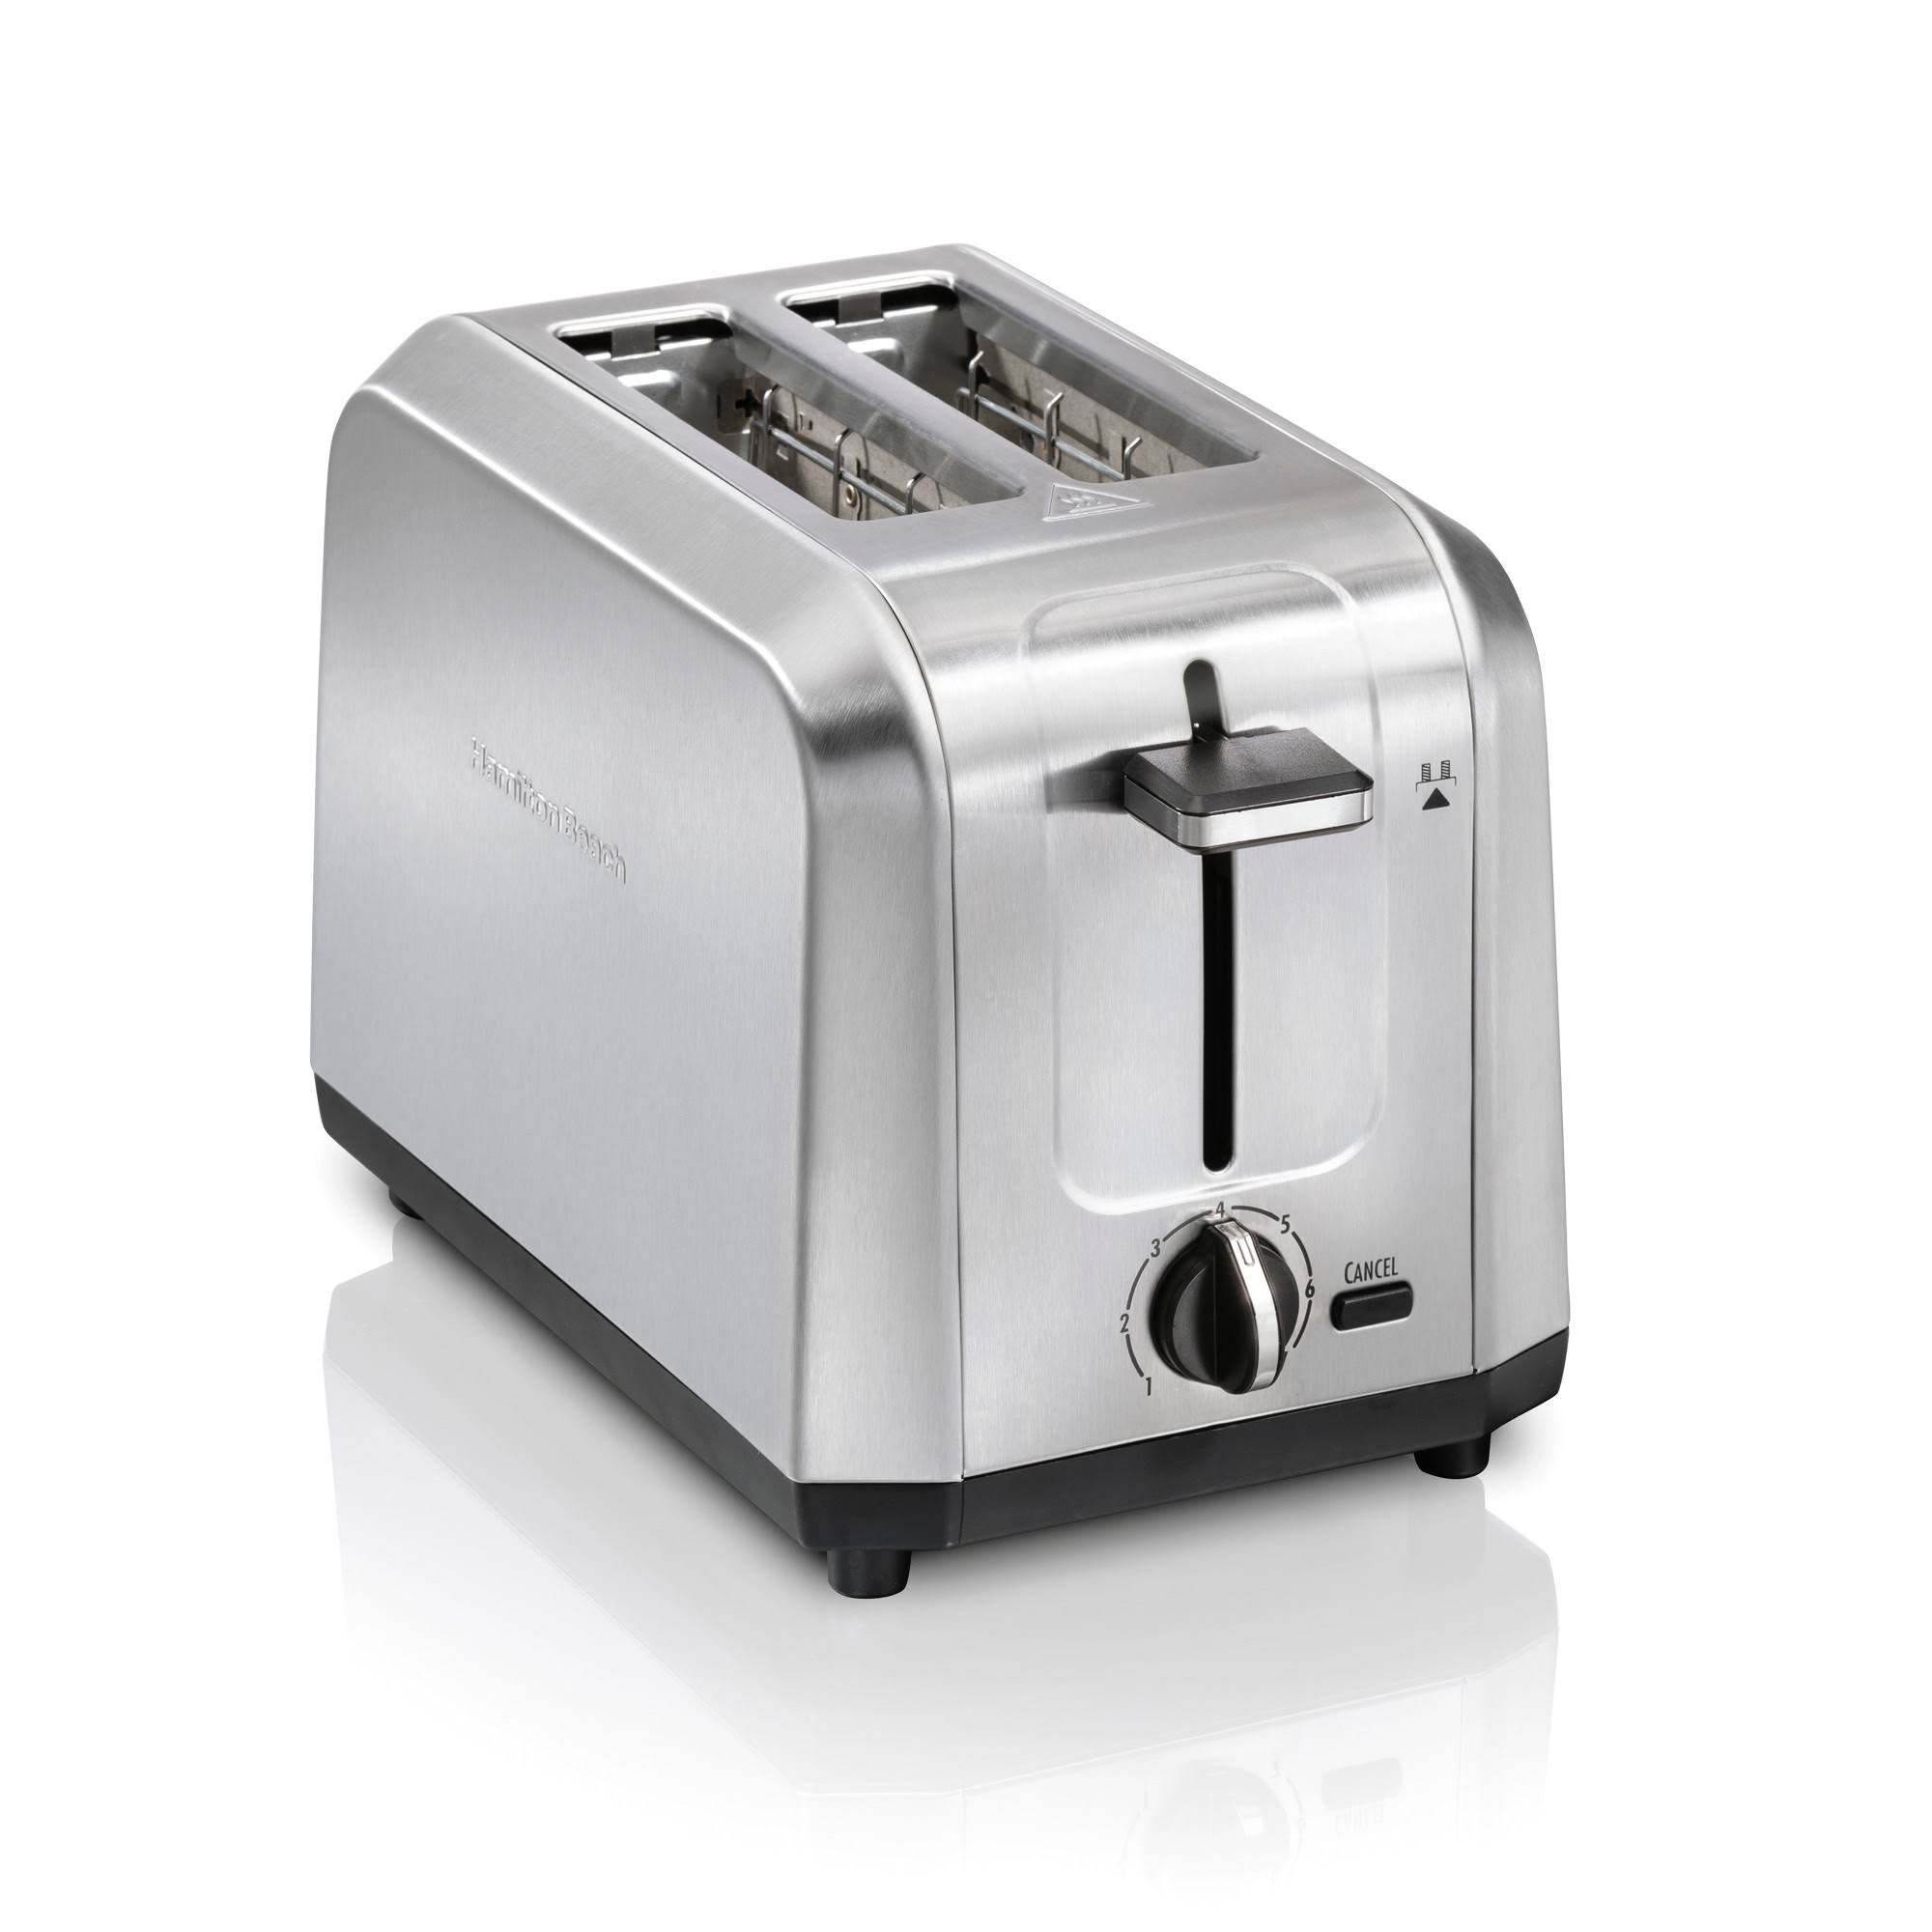
\includegraphics[scale=0.155]{toaster}

  \begin{tabular}{|c|l|}
    \hline
    \(\FR_1\) & Body contains all parts \\
    \hline
    \(\FR_2\) & Can be safely moved while hot \\
    \hline
    \(\FR_3\) & Can hold two slices of bread \\
    \hline
    \(\FR_4\) & Heats each slice of bread on both sides \\
    \hline
    \(\FR_5\) & Toasting is manually started \\
    \hline
    \(\FR_6\) & Toasting is automatically or can be manually stopped \\
    \hline
    \(\FR_7\) & Heat level can be controlled \\
    \hline
  \end{tabular}
  \caption{An example toaster.}
  \label{fig:toaster}
\end{figure}

The graph \(G_1\) for the first candidate design with \(n=7\) and \(m=13\) is shown in
\figurename~\ref{fig:design1}.

\begin{figure}[H]
  \centering
  \scalebox{0.75}{
    \begin{tikzpicture}
      \node [draw,circle] (fr1) at (4,0) {\(\FR_1\)};
      \node [draw,circle] (fr2) at (-1,2) {\(\FR_2\)};
      \node [draw,circle] (fr3) at (0,6) {\(\FR_3\)};
      \node [draw,circle] (fr4) at (1,2) {\(\FR_4\)};
      \node [draw,circle] (fr5) at (0,-4) {\(\FR_5\)};
      \node [draw,circle] (fr6) at (0,-1.5) {\(\FR_6\)};
      \node [draw,circle] (fr7) at (-4,0) {\(\FR_7\)};
      \draw (fr1) edge (fr3);
      \draw (fr1) edge (fr4);
      \draw (fr1) edge (fr5);
      \draw (fr1) edge (fr6);
      \draw (fr1) edge (fr7);
      \draw (fr2) edge (fr3);
      \draw (fr2) edge (fr4);
      \draw (fr2) edge (fr7);
      \draw (fr3) edge (fr4);
      \draw (fr3) edge (fr7);
      \draw (fr5) edge (fr6);
      \draw (fr5) edge (fr7);
      \draw (fr6) edge (fr7);
    \end{tikzpicture}
  }

  \(G_1\)
  \caption{First candidate design.}
  \label{fig:design1}
\end{figure}

When the design tool is run on this first design graph, the graph is found to be \chromatic{4} with the example
chromatic coloring shown in \figurename~\ref{fig:d1color}.

\begin{figure}[H]
  \centering
  \scalebox{0.75}{
    \begin{tikzpicture}
      \colorlet{c1}{green!25!white}
      \colorlet{c2}{blue!25!white}
      \colorlet{c3}{red!25!white}
      \colorlet{c4}{orange!25!white}
      \node [draw,circle,fill=c1] (fr1) at (4,0) {\(\FR_1\)};
      \node [draw,circle,fill=c1] (fr2) at (-1,2) {\(\FR_2\)};
      \node [draw,circle,fill=c3] (fr3) at (0,6) {\(\FR_3\)};
      \node [draw,circle,fill=c2] (fr4) at (1,2) {\(\FR_4\)};
      \node [draw,circle,fill=c4] (fr5) at (0,-4) {\(\FR_5\)};
      \node [draw,circle,fill=c3] (fr6) at (0,-1.5) {\(\FR_6\)};
      \node [draw,circle,fill=c2] (fr7) at (-4,0) {\(\FR_7\)};
      \draw (fr1) edge (fr3);
      \draw (fr1) edge (fr4);
      \draw (fr1) edge (fr5);
      \draw (fr1) edge (fr6);
      \draw (fr1) edge (fr7);
      \draw (fr2) edge (fr3);
      \draw (fr2) edge (fr4);
      \draw (fr2) edge (fr7);
      \draw (fr3) edge (fr4);
      \draw (fr3) edge (fr7);
      \draw (fr5) edge (fr6);
      \draw (fr5) edge (fr7);
      \draw (fr6) edge (fr7);
    \end{tikzpicture}
  }

  \(G_1\)
  \caption{First design chromatic coloring.}
  \label{fig:d1color}
\end{figure}

Notice in the design that \(\FR_5\) (start toasting) and \(\FR_6\) (stop toasting) have been forced into separate
parts, conceivably to accommodate the separate ``cancel'' button shown in \figurename~\ref{fig:toaster}.  But what
if the designer decides to eliminate the cancel button and allow manual cancellation via the lever?  Thus,
\(\FR_5\) and \(\FR_6\) no longer need to be separated, so the edge between their vertices can be eliminated.  The
result is shown in \figurename~\ref{fig:design2}.

\begin{figure}[H]
  \centering
  \scalebox{0.75}{
    \begin{tikzpicture}
      \node [draw,circle] (fr1) at (4,0) {FR1};
      \node [draw,circle] (fr2) at (-1,2) {FR2};
      \node [draw,circle] (fr3) at (0,6) {FR3};
      \node [draw,circle] (fr4) at (1,2) {FR4};
      \node [draw,circle] (fr5) at (0,-4) {FR5};
      \node [draw,circle] (fr6) at (0,-1.5) {FR6};
      \node [draw,circle] (fr7) at (-4,0) {FR7};
      \draw (fr1) edge (fr3);
      \draw (fr1) edge (fr4);
      \draw (fr1) edge (fr5);
      \draw (fr1) edge (fr6);
      \draw (fr1) edge (fr7);
      \draw (fr2) edge (fr3);
      \draw (fr2) edge (fr4);
      \draw (fr2) edge (fr7);
      \draw (fr3) edge (fr4);
      \draw (fr3) edge (fr7);
      \draw (fr5) edge (fr7);
      \draw (fr6) edge (fr7);
    \end{tikzpicture}
  }

  \(G_2\)
  \caption{Second candidate design.}
  \label{fig:design2}
\end{figure}

Now, running the tool indicates that the second design graph is \chromatic{3} with the example coloring shown in
\figurename~\ref{fig:d2color}.

\begin{figure}[H]
  \centering
  \scalebox{0.75}{
    \begin{tikzpicture}
      \colorlet{c1}{green!25!white}
      \colorlet{c2}{blue!25!white}
      \colorlet{c3}{red!25!white}
      \node [draw,circle,fill=c1] (fr1) at (4,0) {FR1};
      \node [draw,circle,fill=c1] (fr2) at (-1,2) {FR2};
      \node [draw,circle,fill=c3] (fr3) at (0,6) {FR3};
      \node [draw,circle,fill=c2] (fr4) at (1,2) {FR4};
      \node [draw,circle,fill=c3] (fr5) at (0,-4) {FR5};
      \node [draw,circle,fill=c3] (fr6) at (0,-1.5) {FR6};
      \node [draw,circle,fill=c2] (fr7) at (-4,0) {FR7};
      \draw (fr1) edge (fr3);
      \draw (fr1) edge (fr4);
      \draw (fr1) edge (fr5);
      \draw (fr1) edge (fr6);
      \draw (fr1) edge (fr7);
      \draw (fr2) edge (fr3);
      \draw (fr2) edge (fr4);
      \draw (fr2) edge (fr7);
      \draw (fr3) edge (fr4);
      \draw (fr3) edge (fr7);
      \draw (fr5) edge (fr7);
      \draw (fr6) edge (fr7);
    \end{tikzpicture}
  }

  \(G_2\)
  \caption{Second design chromatic coloring.}
  \label{fig:d2color}
\end{figure}

This process gives the designer the feedback that the second design requires only three parts instead of four, and
thus has less information content and hence a higher chance of success than the first design.  It will be up to the
designer to weigh this result against other aspects of the design.


\bibliography{thesis}
\bibliographystyle{plain}

\end{document}
